\documentclass[12pt, a4paper, xetex, openany]{book} % twoside, openright
\usepackage[a4paper,left=1.39in,right=1.39in,top=1.85in,bottom=1.85in]{geometry}
\usepackage[colorlinks,bookmarksopen]{hyperref}
\usepackage[svgnames]{xcolor} % Required to specify font color
\usepackage{graphicx} % Required for box manipulation
%\usepackage[hidelinks]{hyperref}
\usepackage{verbatim}
\usepackage{listings}
\usepackage{color}
\usepackage{caption}
\usepackage[none]{hyphenat}
\usepackage{paralist}
\usepackage{perpage}
\usepackage{amsmath}
\usepackage{soul}
\usepackage{tikz}
\usepackage{forest}
\usepackage{tikz-qtree}
\usetikzlibrary{decorations.text}
\usepackage{banglatex}
\usepackage{fontspec}
\usetikzlibrary{shapes,calc,arrows,through,intersections,angles,positioning,quotes,decorations.markings,shapes.multipart,chains}
\usepackage{tkz-euclide}
\usepackage{upquote}
\usepackage{makeidx}
\usepackage{indentfirst}
\usepackage[makeroom]{cancel}
\usetikzlibrary{matrix,arrows,fit}
\usepackage{subcaption}
\usepackage{longtable}
\usetkzobj{all}
\renewcommand{\baselinestretch}{1.1}

%----------------------------------------------------------------------------------------
%   Enable indexing
%----------------------------------------------------------------------------------------
\makeindex
%\newfontfamily{\bengalifonttt}{SolaimanLipi}

%----------------------------------------------------------------------------------------
%   Footnote numbering restarts per page
%----------------------------------------------------------------------------------------
\MakePerPage{footnote}

%----------------------------------------------------------------------------------------
%   Big O
%----------------------------------------------------------------------------------------
\newcommand{\BigO}[1]{\ensuremath{\operatorname{O}\bigl(#1\bigr)}}

\hypersetup{hidelinks=true}

%----------------------------------------------------------------------------------------
%   Space in the page of content
%----------------------------------------------------------------------------------------
\makeatletter
\renewcommand{\l@section}{\@dottedtocline{1}{1.5em}{2.6em}}
\renewcommand{\l@subsection}{\@dottedtocline{2}{4.0em}{3.6em}}
\renewcommand{\l@subsubsection}{\@dottedtocline{3}{7.4em}{4.5em}}
\makeatother

%----------------------------------------------------------------------------------------
%   CODE FORMATTING
%----------------------------------------------------------------------------------------
\definecolor{listinggray}{gray}{0.9}
\definecolor{lbcolor}{rgb}{0.9,0.9,0.9}
\newfontfamily{\lstcourier}[Scale=0.85]{Courier}
\lstset{
    backgroundcolor=\color{lbcolor},
    tabsize=4,
    language=[GNU]C++,
	basicstyle=\lstcourier,
	upquote=true,
	aboveskip={1.5\baselineskip},
	columns=fixed,
	showstringspaces=false,
	extendedchars=false,
	breaklines=true,
	prebreak = \raisebox{0ex}[0ex][0ex]{\ensuremath{\hookleftarrow}},
	frame=single,
	numbers=left,
	showtabs=false,
	showspaces=false,
	showstringspaces=false,
	identifierstyle=\lstcourier,
	keywordstyle=\lstcourier,
	% keywordstyle=\color[rgb]{0,0,1},
	% commentstyle=\color[rgb]{0.0,0.4,0.00},
	% stringstyle=\color[rgb]{0.627,0.126,0.000},
	% numberstyle=\color[rgb]{0.205, 0.142, 0.73},
	xleftmargin=2.5em,
	framexleftmargin=2.5em,
}

%----------------------------------------------------------------------------------------
%	TITLE PAGE
%----------------------------------------------------------------------------------------

\newcommand*{\rotrt}[1]{\rotatebox{90}{#1}} % Command to rotate right 90 degrees
\newcommand*{\rotlft}[1]{\rotatebox{-90}{#1}} % Command to rotate left 90 degrees

\newcommand*{\titleBC}{\begingroup % Create the command for including the title page in the document
\centering % Center all text

\def\CP{\textit{\Huge জিলাটেক ব্যবহার করে বাংলায় টেকনিক্যাল লেখালেখি}} % Title
\def\CCP{\textit{\Huge নমুনা টেমপ্লেট}}

\newlength{\drop} % Command for generating a specific amount of whitespace
\drop=0.1\textheight % Define the command as 10% of the total text height
\rule{\textwidth}{1pt}\par % Thick horizontal line
\vspace{2pt}\vspace{-\baselineskip} % Whitespace between lines
\rule{\textwidth}{0.4pt}\par % Thin horizontal line
\vspace{\drop} % Whitespace between the top lines and title


\settowidth{\unitlength}{\CCP} % Set the width of the curly brackets to the width of the title
{\color{Black}\resizebox*{\unitlength}{\baselineskip}{\rotrt{$\}$}}} \\[\baselineskip] % Print top curly bracket
\textcolor{Black}{\CP} \\[\baselineskip] % Print title
{\color{Black}\Huge নমুনা টেমপ্লেট} \\ % Tagline or further description
{\color{Black}\resizebox*{\unitlength}{\baselineskip}{\rotlft{$\}$}}} % Print bottom curly bracket

%\vfill % Whitespace between the title and the author name
\vspace{0.25\drop} % Whitespace between the title and short horizontal line
\vspace{\drop} % Whitespace between the thin horizontal line and the author name

{\Large\textbf{নিউটন মু. আ. হাকিম (mahnewton@gmail.com)}}\\ % Author name
{\Large\textbf{মোঃ মাহবুবুল হাসান (shanto86@gmail.com)}}\\ % Author name
{\Large\textbf{তাহমিদ রাফি (tahmid.rafi@dimikcomputing.com)}}\\ % Author name

\vfill % Whitespace between the author name and the publisher logo

\vspace*{\drop} % Whitespace under the publisher text
অগাস্ট, ২০১৬ % Year published
\rule{\textwidth}{0.4pt}\par % Thin horizontal line
\vspace{1em} % Whitespace under the publisher text

\includegraphics{image/logo.png}\\[1.27cm]
\vspace{-3em}
{\Large\textbf{দ্বিমিক প্রকাশনী}}\\ % Publisher name
\rule{\textwidth}{0.4pt}\par % Thin horizontal line
\vspace{2pt}\vspace{-\baselineskip} % Whitespace between lines
\rule{\textwidth}{1pt}\par % Thick horizontal line

\endgroup
}

%----------------------------------------------------------------------------------------
%	END TITLE PAGE
%----------------------------------------------------------------------------------------

%%%%%%%%
\begin{document}
\sloppy
\titleBC

%----------------------------------------------------------------------------------------
%	PRINTERS PAGE
%----------------------------------------------------------------------------------------

% Insert printer's page here

%----------------------------------------------------------------------------------------
%	END PRINTERS PAGE
%----------------------------------------------------------------------------------------


\cleardoublepage
\section*{ভূমিকা}
\addtocounter{section}{1}
\vspace{2em}
এই টেমপ্লেট এ দেখানো হয়েছে কেমন করে ল্যাটেক ব্যবহার করে বাংলায় টেকনিক্যাল ব্লগ লেখা যায়। এর জন্য ব্যবহার করা হয়েছে ধারাপাত ডট কম কর্তৃক প্রস্তুতকৃত বাংলা স্টাইল ফাইল। এই ভুমিকার বাকী অংশটুকু অর্থহীন প্লেসহোল্ডার টেক্সট ব্যবহার করে পুরন করা হয়েছে।

অর্থহীন লেখা যার মাঝে আছে অনেক কিছু। হ্যাঁ, এই লেখার মাঝেই আছে অনেক কিছু। যদি তুমি মনে করো, এটা তোমার কাজে লাগবে, তাহলে তা লাগবে কাজে। নিজের ভাষায় লেখা দেখতে অভ্যস্ত হও। মনে রাখবে লেখা অর্থহীন হয়, যখন তুমি তাকে অর্থহীন মনে করো; আর লেখা অর্থবোধকতা তৈরি করে, যখন তুমি তাতে অর্থ ঢালো। যেকোনো লেখাই তোমার কাছে অর্থবোধকতা তৈরি করতে পারে, যদি তুমি সেখানে অর্থদ্যোতনা দেখতে পাও। ...ছিদ্রান্বেষণ? না, তা হবে কেন?

যে কথাকে কাজে লাগাতে চাও, তাকে কাজে লাগানোর কথা চিন্তা করার আগে ভাবো, তুমি কি সেই কথার জাদুতে আচ্ছন্ন হয়ে গেছ কিনা। তুমি যদি নিশ্চিত হও যে, তুমি কোনো মোহাচ্ছাদিত আবহে আবিষ্ট হয়ে অন্যের শেখানো বুলি আত্মস্থ করছো না, তাহলে তুমি নির্ভয়ে, নিশ্চিন্তে অগ্রসর হও। তুমি সেই কথাকে জানো, বুঝো, আত্মস্থ করো; মনে রাখবে, যা অনুসরণ করতে চলেছো, তা আগে অনুধাবন করা জরুরি; এখানে কিংকর্তব্যবিমূঢ় হবার কোনো সুযোগ নেই।

কোনো কথা শোনামাত্রই কি তুমি তা বিশ্বাস করবে? হয়তো বলবে, করবে, হয়তো বলবে "আমি করবো না।" হ্যা, "আমি করবো না" বললেই সবকিছু অস্বীকার করা যায় না, হয়তো তুমি মনের গহীন গভীর থেকে ঠিকই বিশ্বাস করতে শুরু করেছো সেই কথাটি, কিন্তু মুখে অস্বীকার করছো। তাই সচেতন থাকো, তুমি কী ভাবছো- তার প্রতি; সচেতন থাকো, তুমি কি আসলেই বিশ্বাস করতে চলেছো ঐ কথাটি... শুধু এতটুকু বলি, যা-ই বিশ্বাস করো না কেন, আগে যাচাই করে নাও; আর এতে চাই তোমার প্রত্যুৎপন্নমতিত্ব।

তাই কোন কথাটি কাজে লাগবে, তা নির্ধারণ করবে তুমি- হ্যাঁ, তুমি। হয়তো সামান্য ক'টা বাংলা অক্ষর: খন্ড-ত, অনুস্বার, বিঃসর্গ কিংবা চন্দ্রবিন্দু- কিন্তু যদি তুমি বিশ্বাস করো, তাহলে হয়তো তুমি তা দিয়েই তৈরি করতে পারো এক উচ্চমার্গীয় মহাকাব্য- এক চিরসবুজ অর্ঘ্য। রচিত হতে পারে পৃথিবীর ১ম বিরাম চিহ্নের ইতিকথা - এক নতুন ঊষা। ...মহাকাব্য লিখতে ঋষি-মুনি হওয়া লাগে না।
অর্থহীনতা আর অর্থদ্যোতনার সেই ঈর্ষাকাতর মোহাবিষ্টতা তাই তৈরি করে নাও নিজের মাঝে- চাই একটুখানি ঔৎসুক্য। নিজেই ঠিক করো, নিজের ভাষাটা কি অর্থহীন, নাকি কিছু সত্যিই বলছে!

অর্থহীন লেখা যার মাঝে আছে অনেক কিছু। হ্যাঁ, এই লেখার মাঝেই আছে অনেক কিছু। যদি তুমি মনে করো, এটা তোমার কাজে লাগবে, তাহলে তা লাগবে কাজে। নিজের ভাষায় লেখা দেখতে অভ্যস্ত হও। মনে রাখবে লেখা অর্থহীন হয়, যখন তুমি তাকে অর্থহীন মনে করো; আর লেখা অর্থবোধকতা তৈরি করে, যখন তুমি তাতে অর্থ ঢালো। যেকোনো লেখাই তোমার কাছে অর্থবোধকতা তৈরি করতে পারে, যদি তুমি সেখানে অর্থদ্যোতনা দেখতে পাও। ...ছিদ্রান্বেষণ? না, তা হবে কেন?

যে কথাকে কাজে লাগাতে চাও, তাকে কাজে লাগানোর কথা চিন্তা করার আগে ভাবো, তুমি কি সেই কথার জাদুতে আচ্ছন্ন হয়ে গেছ কিনা। তুমি যদি নিশ্চিত হও যে, তুমি কোনো মোহাচ্ছাদিত আবহে আবিষ্ট হয়ে অন্যের শেখানো বুলি আত্মস্থ করছো না, তাহলে তুমি নির্ভয়ে, নিশ্চিন্তে অগ্রসর হও। তুমি সেই কথাকে জানো, বুঝো, আত্মস্থ করো; মনে রাখবে, যা অনুসরণ করতে চলেছো, তা আগে অনুধাবন করা জরুরি; এখানে কিংকর্তব্যবিমূঢ় হবার কোনো সুযোগ নেই।

কোনো কথা শোনামাত্রই কি তুমি তা বিশ্বাস করবে? হয়তো বলবে, করবে, হয়তো বলবে "আমি করবো না।" হ্যা, "আমি করবো না" বললেই সবকিছু অস্বীকার করা যায় না, হয়তো তুমি মনের গহীন গভীর থেকে ঠিকই বিশ্বাস করতে শুরু করেছো সেই কথাটি, কিন্তু মুখে অস্বীকার করছো। তাই সচেতন থাকো, তুমি কী ভাবছো- তার প্রতি; সচেতন থাকো, তুমি কি আসলেই বিশ্বাস করতে চলেছো ঐ কথাটি... শুধু এতটুকু বলি, যা-ই বিশ্বাস করো না কেন, আগে যাচাই করে নাও; আর এতে চাই তোমার প্রত্যুৎপন্নমতিত্ব।

তাই কোন কথাটি কাজে লাগবে, তা নির্ধারণ করবে তুমি- হ্যাঁ, তুমি। হয়তো সামান্য ক'টা বাংলা অক্ষর: খন্ড-ত, অনুস্বার, বিঃসর্গ কিংবা চন্দ্রবিন্দু- কিন্তু যদি তুমি বিশ্বাস করো, তাহলে হয়তো তুমি তা দিয়েই তৈরি করতে পারো এক উচ্চমার্গীয় মহাকাব্য- এক চিরসবুজ অর্ঘ্য। রচিত হতে পারে পৃথিবীর ১ম বিরাম চিহ্নের ইতিকথা - এক নতুন ঊষা। ...মহাকাব্য লিখতে ঋষি-মুনি হওয়া লাগে না।
অর্থহীনতা আর অর্থদ্যোতনার সেই ঈর্ষাকাতর মোহাবিষ্টতা তাই তৈরি করে নাও নিজের মাঝে- চাই একটুখানি ঔৎসুক্য। নিজেই ঠিক করো, নিজের ভাষাটা কি অর্থহীন, নাকি কিছু সত্যিই বলছে!

অর্থহীন লেখা যার মাঝে আছে অনেক কিছু। হ্যাঁ, এই লেখার মাঝেই আছে অনেক কিছু। যদি তুমি মনে করো, এটা তোমার কাজে লাগবে, তাহলে তা লাগবে কাজে। নিজের ভাষায় লেখা দেখতে অভ্যস্ত হও। মনে রাখবে লেখা অর্থহীন হয়, যখন তুমি তাকে অর্থহীন মনে করো; আর লেখা অর্থবোধকতা তৈরি করে, যখন তুমি তাতে অর্থ ঢালো। যেকোনো লেখাই তোমার কাছে অর্থবোধকতা তৈরি করতে পারে, যদি তুমি সেখানে অর্থদ্যোতনা দেখতে পাও। ...ছিদ্রান্বেষণ? না, তা হবে কেন?

যে কথাকে কাজে লাগাতে চাও, তাকে কাজে লাগানোর কথা চিন্তা করার আগে ভাবো, তুমি কি সেই কথার জাদুতে আচ্ছন্ন হয়ে গেছ কিনা। তুমি যদি নিশ্চিত হও যে, তুমি কোনো মোহাচ্ছাদিত আবহে আবিষ্ট হয়ে অন্যের শেখানো বুলি আত্মস্থ করছো না, তাহলে তুমি নির্ভয়ে, নিশ্চিন্তে অগ্রসর হও। তুমি সেই কথাকে জানো, বুঝো, আত্মস্থ করো; মনে রাখবে, যা অনুসরণ করতে চলেছো, তা আগে অনুধাবন করা জরুরি; এখানে কিংকর্তব্যবিমূঢ় হবার কোনো সুযোগ নেই।

কোনো কথা শোনামাত্রই কি তুমি তা বিশ্বাস করবে? হয়তো বলবে, করবে, হয়তো বলবে "আমি করবো না।" হ্যা, "আমি করবো না" বললেই সবকিছু অস্বীকার করা যায় না, হয়তো তুমি মনের গহীন গভীর থেকে ঠিকই বিশ্বাস করতে শুরু করেছো সেই কথাটি, কিন্তু মুখে অস্বীকার করছো। তাই সচেতন থাকো, তুমি কী ভাবছো- তার প্রতি; সচেতন থাকো, তুমি কি আসলেই বিশ্বাস করতে চলেছো ঐ কথাটি... শুধু এতটুকু বলি, যা-ই বিশ্বাস করো না কেন, আগে যাচাই করে নাও; আর এতে চাই তোমার প্রত্যুৎপন্নমতিত্ব।


\tableofcontents

%for book the following things might help
%\begin{titlepage}
% design your title page here
%\end{titlepage}
%\resetbengalipage
%\bengalipageplainalpha
%\tableofcontents
%\listoffigures
%\clearpage
%\resetbengalipage
%\bengalipagefancynumber
%\fancyhead[LO,RE]{\sl\nouppercase\leftmark} % twoside
%\fancyhead[LE,RO]{\sl\nouppercase\rightmark} % twoside

\chapter{ইন্সটলেশন সংক্রান্ত তথ্যাদি}

\section{সুচনা}

আগে লাটেক (LaTeX) পরিবারে সরাসরি বাংলায় টাইপ সেটিংয়ের সহজ উপায় ছিল না। তবে কিছু দিন আগে থেকে ব্যাংটেক (bangtex) ব্যবহৃত হয়ে আসছে। কিন্তু ব্যাংটেক ব্যবহার করা বেশ কঠিন। সরাসরি বাংলা অক্ষরে লিখতে না পারলে আমরা যেমন ইংলিশ অক্ষরে বাংলা লিখে থাকি যেমন "emon deshti kothao khuje pabe nako tumi, sokol desher ranee se je amar jonmo vumi", ব্যাংটেকে বাংলা টাইপ সেটিং করতে গেলে ঠিক সেরকমটি করতে হয়। বাংলা শব্দগুলো ইংলিশ অক্ষরে লিখে সাথে যুক্তাক্ষর সহ অন্যান্য বিষয়াদি সোর্স ফাইলে বিশেষ ধরনের সংকেতে দিয়ে দিতে হয়। এরপর ব্যাংটেক ও ল্যাটেকের প্রোগ্রাম দিয়ে আপনার সোর্স ফাইল কম্পাইল করলে বাংলায় টাইপ সেটিং হয়ে আউটপুট ফাইলটি পাওয়া যায়। 

সাম্প্রতিক কালে জিলাটেকের (XeLaTeX) এর আগমনে বাংলায় টাইপ সেটিং সহজ হয়ে গিয়েছে। জিলাটেকের কল্যানে আপনি আপনার সোর্স টেক (.tex) ফাইলে সরাসরি ইউনিকোডে বাংলা লিখতে পারবেন। একাজে ইউনিকোড সাপোর্ট করে আপনার পছন্দের এরকম যেকোন এডিটর প্রোগ্রাম ব্যবহার করুন। তারপর জিলাটেক প্রোগ্রাম দিয়ে আপনার সোর্স ফাইলটিকে কম্পাইল করতে হবে। আসলে জিলাটেক দিয়ে আরো অনেক ভাষায়ই সরাসরি টাইপ সেটিং করা যায়, তবে আমরা এখানে শুধু বাংলায় টাইপ সেটিং নিয়ে কথা বলব। জিলাটেকের সাথে ব্যবহারের জন্য পলিগ্লোসিয়া (polyglossia.sty) নামক একটি স্টাইল ফাইল দরকার হয়। এই স্টাইল ফাইলটি ইংলিশের পরিবর্তে বাংলা ব্যবহৃত হলে যেসব অনুবাদের দরকার হয় সেই কাজগুলো করে। যেমন ইংলিশ চ্যাপ্টারের বদলে অধ্যায়, ইংলিশ ডিজিটের বদলে বাংলা অঙ্ক, ইংলিশ মাসের নামের বদলে বাংলায় মাসের নাম, ইত্যাদি। তবে জিলাটেক ও পলিগ্লোসিয়ার এই কম্বিনেশন আসলে সম্পূর্ণ নয়, এটা শুধু আপনার লেখার মুল কথাবার্তাগুলোর দিকে নজর দেয়। কিন্তু অনেক খুঁটিনাটি বিষয় যেমন পৃষ্ঠা, অধ্যায়, পরিচ্ছেদ, অনুচ্ছেদ, ইত্যাদির ক্রমিক সহ আরো অনেককিছু বাংলায় আসে না। তাছাড়া গুরুত্ব বজার রেখে বাংলা ফন্ট নির্ধারণের বিষয়েও ঐ কম্বিনেশন থেকে আপনি কোন ধারণা পাবেন না। সব মিলিয়ে মোটা দাগেও সন্তোষ্টি অর্জন একটু কঠিন হয়ে যায়।  

জিলাটেক ও পলিগ্লোসিয়ার উপরে বর্ণিত অসম্পূর্ণতা গুলো বেশ খানিকটা দুর করার জন্য আমরা নতুন দুটো স্টাইল ফাইল বানিয়েছি: একটা হল জিলাটেকবেংগলি (xelatexbengali.sty) আরেকটি হল বেংগলিডিজিটস (bengalidigits.sty)। এই লেখায় আমরা এই স্টাইল ফাইলগুলো নিয়ে আলোচনা করেছি। আমাদের তৈরী বেংগলিডিজিটস স্টাইল ফাইলটি ইংলিশ লেটার বা ডিজিটের বদলে বাংলা অক্ষর বা অঙ্ক পেতে সাহায্য করে। আর জিলাটেকবেংগলি স্টাইল ফাইলটি আরেকটু হাই লেভেলে কোন ইংলিশ শব্দের বদলে কোন বাংলা শব্দ ব্যবহার করতে হবে, বা কোনখানে কোন ফন্ট ব্যবহৃত হবে, অথবা অধ্যায়, পরিচ্ছেদ, অনুচ্ছেদ, ইত্যাদির ক্রমিক নম্বর ঠিক কীভাবে দেখানো হবে এসব নির্ধারন করে। আপনি যদি এ সবে কোন পরিবর্তন করতে চান তাহলে জিলাটেকবেংগলি স্টাইল ফাইলটি পরিবর্তন করে নিতে পারবেন, তবে বেংগলিডিজিটসে আপনার কোন পরিবর্তনের দরকার হবে বলে মনে হয় না।  

সব মিলিয়ে আপনার কাজের সুবিধার জন্য এই লেখার পিডিএফ ফাইলের সাথে আমরা আমাদের তৈরী স্টাইলফাইল গুলোসহ আরো দরকারী অন্যান্য ফাইল দিয়ে দিয়েছি। আর এই লেখায় পরের দিকে ইন্সটলেশন প্রসিডিউর ও ব্যবহারের নিয়মকানুন বর্ণনা করা হয়েছে। আপনি চাইলে ‌\cite{thisdoc} থেকেও এই বিষয়ে  আলোচনা পেতে পারেন।\footnote{এটা আসলে এই নিবন্ধেরই যোগসুত্র, স্রেফ তথ্যসুত্র ও পাদটিকার উদাহরণ হিসাবে এটি দেখানো হয়েছে।} এছাড়া আমরা sample.tex নামক একটা সোর্স টেক (.tex) ফাইল দিয়েছি যেটিকে আপনি চাইলে জিলাটেক দিয়ে বাংলা টাইপ সেটিংয়ের একটা উদাহরণ হিসাবে ব্যবহার করতে পারবেন। 

\section{ইন্সটলেশন প্রসিডিউর}

আমাদের জিলাটেকবেংগলি ও বেংগলিডিজিটস স্টাইল ফাইলদুটো আর সাথে দরকারী আরো ফাইলগুলোর তালিকা \tablename~\ref{thistable} এ দেয়া হল। এছাড়া ইন্সটলেশন প্রসিডিউরও আমরা নীচে বর্ণনা করছি। তবে আমরা এখানে কেবল উইনডোজের মিকটেক (MiKTeX) এবং উবুন্তু অপারেটিং সিস্টেমের জন্য ইন্সটলেশন ব্যাখ্যা করব। আপনি যদি নিজে অন্য কোন অপারেটিং সিস্টেমে সফল ভাবে ব্যবহার করতে পারেন, তাহলে ইন্সটলেশনের একটা খসড়া বর্ণনা আমাদের দিতে পারেন, আমরা আপনার নামসহ সেই বর্ণনা এইখানে যোগ করে দিব। 

\begin{table}[!hbt]
	\caption{ফাইলগুলোর তালিকা\label{thistable}}
	\begin{center}\begin{footnotesize}
	\begin{tabular}{|l|l|}
		\hline
		polyglossia.sty & জিলাটেকে বিভিন্ন ভাষা ব্যবহারের মুল স্টাইল ফাইল‌‌\\\hline
		xelatexbengali.sty & জিলাটেকে বাংলা টাইপ সেটিংয়ের মুল স্টাইল ফাইল\\\hline
		beamerthemexelatexbengali.sty & জিলাটেকে বিমার দিয়ে প্রেজেন্টেশনের জন্য মুল ফাইল।\\\hline 
		gloss-bengali.ldf & পলিগ্লোসিয়া স্টাইলে বাংলা সাপোর্টের জন্য দরকারী ফাইল\\\hline
		bengalidigits.sty & ইংলিশ থেকে বাংলায় অক্ষর ও অঙ্ক অনুবাদের জন্য দরকারী\\\hline
		bengalidigits.map &	 \begin{minipage}{0.5\textwidth}ইংলিশ থেকে বাংলায় বদল সংক্রান্ত, তবে নিশ্চিত নয়\end{minipage}\\\hline
		bengalidigits.tec & \begin{minipage}{0.5\textwidth}ইংলিশ থেকে বাংলায় বদল সংক্রান্ত, তবে নিশ্চিত নয়\end{minipage}\\\hline
               সাতটি .ttf ফন্ট ফাইল & \begin{minipage}{0.5\textwidth}একুশে আজাদ, একুশে দুর্গা, একুশে পূণর্ভবা, রুপালি, একুশে স্বরস্বতী, সোলায়মানলিপি, সোলায়মানলিপি জোর\end{minipage}\\\hline
	\end{tabular}
	\end{footnotesize}\end{center}
\end{table}

\subsection{সহজ পদ্ধতি}
আমরা জানি ল্যাটেক পরিবারের বিভিন্ন স্টাইল ফাইলগুলো আমাদের কারেন্ট ফোল্ডারে রাখলেই চলে। এই পদ্ধতি অনুসারে আমাদের দেয়া সকল ফাইল আপনার যে ফোল্ডারে .tex ফাইলটিকে রাখবেন সেখানে কপি পেস্ট করে দিন। তবে নীচের উবুন্ত ও উইনডোজের জন্য আমাদের দেয়া ১ নম্বর ধাপ গুলো অনুসরণ করে আপনাকে দরকারমতো যথাক্রমে লাটেক ও মিকটেক ইন্সটল করতে হবে। তারপর ৪ নম্বর ধাপ অনুসরণ করে ফন্টও ইন্সটল করতে হবে। 
\subsection{উবুন্তু অপারেটিং সিস্টেম}

\begin{enumerate}
\item আপনার কম্পিউটারের উবুন্তু অপারেটিং সিস্টেমে গিয়ে লাটেক ও জিলাটেক ইন্সটল করুন। যদি আগে থেকে করা থাকে, তাহলে তো কথাই নেই। আর না থাকলে আপনি টার্মিনাল ওপেন করে কমান্ডপ্রোম্পটে নীচের কমান্ডগুলো দিয়ে লাটেক ও জিলাটেক ইন্সটল করুন। 
\begin{itemize}
\item sudo apt-get install texlive
\item sudo apt-get install texlive-latex-extra
\item sudo apt-get install texlive-xetex
\item sudo apt-get install latex-beamer (প্রেজেন্টেশন বানাতে চাইলে)
\end{itemize}

বিকল্প হিসাবে আপনি উবুন্তু সফটওয়্যার সেন্টারে গিয়েও তা করতে পারবেন।
\item এখন আপনার ফোল্ডার ট্রিতে পলিগ্লোসিয়া স্টাইল polyglossia.sty ফাইলটি খুঁজে বের করুন। এই ফাইলটি জিলাটেকের সাথেই ইন্সটল হয়ে যাওয়ার কথা। আর সেক্ষেত্রে খুব সম্ভবত এই ফাইলটি নীচের পাথে থাকবে।
\begin{quote}/usr/share/texlive/texmf-dist/tex/xelatex/polyglossia\end{quote}

এবার টার্মিনালের কমান্ড প্রোম্পটে গিয়ে ls কমান্ড চালিয়ে ঐ পাথে অনেক ফাইলের সাথে যে ফাইলগুলো দেখতে পাবেন সেগুলো হলো: \begin{quote}polyglossia.sty\end{quote} \begin{quote}অনেকগুলো gloss-<scriptname>.ldf\end{quote} \begin{quote}devanagaridigits.sty\end{quote} এবার আপনি আমাদের দেয়া   
\begin{quote}polyglossia.sty\end{quote}\begin{quote}gloss-bengali.ldf\end{quote}\begin{quote}bengalidigits.sty\end{quote}\begin{quote}xelatexbengali.sty\end{quote} \begin{quote}beamerthemexelatexbengali.sty\end{quote} ফাইল পাঁচটি ঐ ফোল্ডারে কপি করে দিন। এই ফাইলগুলো যদি ঐ ফোল্ডারে আগে থেকেই থাকে তাহলে সেগুলোকে রিপ্লেস করে আমাদের গুলো কপি করে দিন। দরকার হলে রিপ্লেস করার আগে আগের ফাইলগুলোকে ভিন্ন নামে কপি করে রাখতে পারেন, যাতে কোন বিপদে পড়লে সেই কপি কাজে লাগানো যায়। তবে এই ফাইলগুলো ঐ ফোল্ডারে কপি করার জন্য আপনার সুডু অ্যাক্সেস (sudo access) লাগতে পারে। ফাইল কপি করা হয়ে গেলে টার্মিনালের কমান্ড প্রোম্পটেই texhash কমান্ডটি কোন প্যারামিটার ছাড়া রান করুন, এক্ষেত্রেও সুডু অ্যাক্সেস লাগতে পারে।

\item আমরা ঠিক নিশ্চিত নই এই ধাপটি অনুসরণ করতে হবে কিনা, তবুও রিকমেন্ড করছি। আমাদের দেয়া bengalidigits.tec ও bengalidigits.map ফাইলদুটো নীচের দুটো পাথে কপি করে দিন।  ফোল্ডার না থাকলে তৈরী করে নিন।
\begin{scriptsize}\begin{quote}‌/usr/share/texlive/texmf-dist/fonts/misc/xetex/fontmapping/xetex-bengali/\end{quote}\end{scriptsize}\begin{scriptsize}\begin{quote}/usr/share/texlive/texmf-dist/fonts/misc/xetex/fontmapping/polyglossia/\end{quote}\end{scriptsize}
ঐ পাথগুলো বা ঐ ফাইলগুলো যদি আগে থেকেই থাকে তাহলে অবশ্য আর কপি করার দরকার নেই। আর যদি কপি করতেই চান তাহলে আগের গুলোকে ভিন্ন নামে কপি করে রাখুন, যাতে কোন বিপদে পড়লে সেগুলো কাজে লাগাতে পারেন।

\item এবার আমাদের দেয়া সাতটি ফন্ট ইন্সটল করুন। ফন্টগুলো হল একুশে আজাদ, একুশে দুর্গা, একুশে পুনর্ভবা, রুপালী, একুশে স্বরস্বতী, সোলায়মানলিপি ও সোলায়মানলিপি জোর। এগুলো মুক্ত ফন্ট আর ফ্রীতে পাওয়া যায়। আপনার যদি অনুমতিপত্র বা লাইসেন্স দরকার হয় তাহলে নীচের স্থানদুটো থেকে তা যোগাড় করুন। ‌\begin{quote}http://onkur.sourceforge.net\end{quote}\begin{quote}ekushey.org\end{quote} ফন্ট ইন্সটল করার জন্য আপনাকে fontviewer নামক প্রোগ্রামটি রান করতে হবে। এক এক করে প্রত্যকটি ফন্ট ফন্টভিউয়ার দিয়ে ওপেন করুন। ঐ প্রোগ্রাম রান করলে যে উইন্ডো আসবে তার ডান পাশে উপরের দিকে থাকা একটা বাটনে ক্লিক করে আপনি ফন্টটিকে ইন্সটল করতে পারবেন। আপনার কম্পিউটারে যদি আগে থেকে এই ফন্টগুলোর কোন ভার্সন থাকে সেগুলো পুরনো হতে পারে তাই সেগুলো রিমুভ করে আমাদের গুলো ইন্সটল করুন। বিকল্প হিসাবে আপনার লোকাল বা সিস্টেম ফন্ট ফোল্ডারে ফন্ট ফাইলগুলো কপি করে দিন। আপনার লোকাল ফন্ট ফোল্ডার হল  ‌\begin{quote}$\sim$/.local/share/fonts \end{quote} আর সিস্টেম ফন্ট ফোল্ডার হল ‌\begin{quote}/usr/share/fonts\end{quote} \begin{quote}/usr/local/share/fonts\end{quote} ফন্ট ইন্সটল করার পরে আপনাকে fc-cache প্রোগ্রামটি টার্মিনালের কমান্ড প্রোম্পটে রান করতে হবে, এখানে সুডু অ্যাক্সেস লাগতে পারে।
\end{enumerate}

উপরের ধাপ গুলো সম্পন্ন করলে আপনার কম্পিউটারের উবুন্তু অপারেটিং সিস্টেমে আমাদের দরকারী ইন্সটলেশন কাজ সম্পূর্ণ শেষ! এবার টাইপ সেটিংয়ের পালা। পরের পরিচ্ছেদে তা আলোচনা করা হয়েছে।

\subsection{উইনডোজের জন্য মিকটেক}

\begin{enumerate}
\item আপনার কম্পিউটারের উইনডোজ অপারেটিং সিস্টেমে গিয়ে মিকটেক (MiKTeX) ইন্সটল করুন। যদি আগে থেকে করা থাকে, তাহলে তো কথাই নেই। মিকটেক ইন্সটল করলে লাটেক, জিলাটেক, বিমার সহ দরকারী সবকিছু ইন্সটল হয়ে যাওয়ার কথা। ধরা যাক আপনার মিকটেক ফোল্ডার হল C:\textbackslash{}Program Files\textbackslash{}MiKTeX 2.9। এই পাথটি আপনার মিকটেকের ভার্সনের (যেমন 2.9) উপরের নির্ভর করবে। 
\item এখন আপনার ফোল্ডার ট্রিতে পলিগ্লোসিয়া স্টাইল polyglossia.sty ফাইলটি খুঁজে বের করুন। এই ফাইলটি মিকটেকের সাথেই ইন্সটল হয়ে যাওয়ার কথা। আর সেক্ষেত্রে খুব সম্ভবত এই ফাইলটি নীচের পাথে থাকবে।
\begin{quote}C:\textbackslash{}Program Files\textbackslash{}MikTeX 2.9\textbackslash{}tex\textbackslash{}xelatex\textbackslash{}polyglossia\end{quote} কোন কোন কম্পিউটারে উপরের পাথে না থেকে নীচের এই পাথেও থাকতে পারে, তফাৎ শুধু xelatex এর বদলে latex। \begin{quote}C:\textbackslash{}Program Files\textbackslash{}MikTeX 2.9\textbackslash{}tex\textbackslash{}latex\textbackslash{}polyglossia\end{quote}এবার কমান্ড প্রোম্পটে (start menu থেকে run এ গিয়ে cmd চালালে যে উইন্ডো আসে) গিয়ে dir কমান্ড চালিয়ে ঐ পাথে অনেক ফাইলের সাথে যে ফাইলগুলো দেখতে পাবেন সেগুলো হলো: \begin{quote}polyglossia.sty\end{quote} \begin{quote}অনেকগুলো gloss-<scriptname>.ldf\end{quote} \begin{quote}devanagaridigits.sty\end{quote} এবার আপনি আমাদের দেয়া  \begin{quote}polyglossia.sty\end{quote}\begin{quote}gloss-bengali.ldf\end{quote} \begin{quote}bengalidigits.sty\end{quote} \begin{quote}xelatexbengali.sty\end{quote}\begin{quote}beamerthemexelatexbengali.sty\end{quote} ফাইল পাঁচটি ঐ ফোল্ডারে কপি করে দিন। এই ফাইলগুলো যদি ঐ ফোল্ডারে আগে থেকেই থাকে তাহলে সেগুলোকে রিপ্লেস করে আমাদের গুলো কপি করে দিন। দরকার হলে রিপ্লেস করার আগে আগের ফাইলগুলোকে ভিন্ন নামে কপি করে রাখতে পারেন, যাতে কোন বিপদে পড়লে সেই কপি কাজে লাগানো যায়। ফাইল কপি করা হয়ে গেলে কমান্ড প্রোম্পটে গিয়ে  texhash অথবা mktexlsr অথবা initexmf --update-fndb এই তিনটি কমান্ডের যেকোন একটি অথবা সবগুলো একে একে চালান। বিকল্প হিসাবে start menu থেকে MiKTeX খুঁজে বের করে সেখানে Maintenance (Admin) মেনুতে settings (Admin) চালান। তারপর General ট্যাবে Refresh FNDB বাটনে মাউস ক্লিক করুন। আমরা সবরকম অপশন দিয়ে দিলাম, কোন না কোনটি কাজ করার কথা।
\item আমরা ঠিক নিশ্চিত নই এই ধাপটি অনুসরণ করতে হবে কিনা, তবুও রিকমেন্ড করছি। আমাদের দেয়া bengalidigits.tec ও bengalidigits.map ফাইলদুটো নীচের দুটো পাথে কপি করে দিন।  ফোল্ডার না থাকলে তৈরী করে নিন।
\begin{scriptsize}\begin{quote}‌C:\textbackslash{}Program Files\textbackslash{}MiKTeX 2.9\textbackslash{}fonts\textbackslash{}misc\textbackslash{}xetex\textbackslash{}fontmapping\textbackslash{}xetex-bengali\end{quote}\end{scriptsize}\begin{scriptsize}\begin{quote}C:\textbackslash{}Program Files\textbackslash{}MiKTeX 2.9\textbackslash{}fonts\textbackslash{}misc\textbackslash{}xetex\textbackslash{}fontmapping\textbackslash{}polyglossia\end{quote}\end{scriptsize}
ঐ পাথগুলো বা ঐ ফাইলগুলো যদি আগে থেকেই থাকে তাহলে অবশ্য আর কপি করার দরকার নেই। আর যদি কপি করতেই চান তাহলে আগের গুলোকে ভিন্ন নামে কপি করে রাখুন, যাতে কোন বিপদে পড়লে সেগুলো কাজে লাগাতে পারেন।

\item এবার আমাদের দেয়া সাতটি ফন্ট ইন্সটল করুন। ফন্টগুলো হল একুশে আজাদ, একুশে দুর্গা, একুশে পুনর্ভবা, রুপালী, একুশে স্বরস্বতী, সোলায়মানলিপি ও সোলায়মানলিপি জোর। এগুলো মুক্ত ফন্ট আর ফ্রীতে পাওয়া যায়। আপনার যদি অনুমতিপত্র বা লাইসেন্স দরকার হয় তাহলে নীচের স্থানদুটো থেকে তা যোগাড় করুন। ‌\begin{quote}http://onkur.sourceforge.net\end{quote}\begin{quote}ekushey.org\end{quote} ফন্ট ইন্সটল করার Control Panel থেকে সম্ভবত Appearance and Themes থেকে Fonts খুঁজে বের করতে হবে। এরপর Fonts ফোল্ডার ওপেন হলে আপনাকে আমাদের দেয়া সাতটি ফন্ট কপি-পেস্ট করে দিতে হবে। আপনার কম্পিউটারে যদি আগে থেকে এই ফন্টগুলোর কোন ভার্সন থাকে সেগুলো পুরনো হতে পারে তাই সেগুলো রিমুভ করে আমাদের গুলো ইন্সটল করুন। 
\end{enumerate}

উপরের ধাপ গুলো সম্পন্ন করলে আপনার উইনডোজ কম্পিউটারে আমাদের দরকারী ইন্সটলেশন কাজ সম্পূর্ণ শেষ! এবার টাইপ সেটিংয়ের পালা। পরের পরিচ্ছেদে তা আলোচনা করা হয়েছে।


\section{বাংলা ফন্ট ও টাইপ সেটিং}

আগেই বলেছি জিলাটেক ব্যবহারের ক্ষেত্রে আপনি যা বাংলায় লিখবেন তা সরাসরি ইউনিকোডে বাংলায়ই লিখবেন। এ কাজে ইউনিকোড সাপোর্ট করে আপনার পছন্দের এরকম যে কোন এডিটর প্রোগ্রাম ব্যবহার করুন। আর স্বাভাবিক ভাবে ইংলিশ টাইপসেটিংয়ের জন্য আপনি যে ভাবে লাটেক ব্যবহার করেন, বাংলা টাইপ সেটিংয়ের জন্য সেই একই ভাবেই করবেন। মোটামুটি ভাবে সকল লাটেক কমান্ড জিলাটেকেও কাজ করবে। তবে আপনার সোর্স টেক (.tex) ফাইলটিকে কম্পাইল করার ক্ষেত্রে লাটেকের বদলে জিলাটেক ব্যবহার করতে হবে।  

‌\subsection{বাংলা ফন্ট বিষয়ে মন্তব্য}
আমাদের জিলাটেকবেংগলি স্টাইল xelatexbengali.sty ফাইলে আমরা সাতটি বাংলা ফন্ট ফেস ব্যবহার করেছি। বাংলা ভাষায় ফন্টগুলোর ক্ষেত্রে আসলে সম্পূর্ণতার অভাব দেখা যায়। অনেক সুন্দর ফন্ট ফেস আছে যেটা প্রশংসনীয়। তবে কোন একটা ফন্ট ফ্যামিলির জন্য যতগুলো ভার্সন দরকার তার সবগুলো পাওয়া যায় না বলে মনে হয়। যেমন একটা ফন্টের রেগুলার, বোল্ড, ইটালিক, স্ল্যান্ট, বোল্ড ইটালিক, ইত্যাদি ভার্সন মিলিয়ে একটা ফন্ট ফ্যামিলি তৈরী হবে, এরকমটি নেই। যারা নতুন নতুন বাংলা ফন্ট তৈরী করেন অথবা যারা পুরনো ফন্টগুলোর সংস্কার করছেন, তারা এ বিষয়ে নজর দিলে ভাল হয়। ভিন্ন ভিন্ন ফ্যামিলির ফন্ট নিয়ে টাইপ সেটিংয়ে বেশ কিছু সমস্যা হয়। যেমন এক ফন্টের বাংলা অক্ষরগুলোর মাত্রা যে বরারর, অন্য ফন্টের অক্ষর গুলোর মাত্রা তার চেয়ে উপরে বা নীচে। এছাড়া অক্ষরগুলোর আকারেও ছোট বড় রয়েছে, তবে এই বড় ছোট অবশ্য খানিকটা সমাধান করা যায় স্কেলিং করে। আমাদের অবশ্য আপাতত কিছু করার নেই, ফন্ট বানানো সম্ভব হচ্ছে না। পরে কখনো সুবিধাজনক ফন্ট পাওয়া গেলে সেটা বিবেচনায় নিতে হবে। আপাতত আমরা চেষ্টা করেছি এইগুলো কোন ভাবে ম্যানেজ করতে।

\subsection{ব্যবহৃত বাংলা ফন্ট}
যেমনটি মন্তব্যে বলেছি, যথোপযুক্ত ফন্ট ফ্যামিলির অভাবে আমরা আপাতত বিভিন্ন রকমের ফন্ট ফেস একসাথে ব্যবহার করছি। ইংলিশ টাইপ সেটিংয়ে আমরা যেমন গুরুত্ব বজায় রেখে টাইপ সেটিং করতে পারি, বাংলায়ও আমরা চেষ্টা করব সেরকমটা করতে। এ কাজে আমরা বাজারে বিদ্যমান সাতটি ফন্ট ফেস ব্যবহার করছি। এই ফন্ট ফেসগুলো হল সোলায়মানলিপি, সোলায়মানলিপি বোল্ড, একুশে দুর্গা, একুশে পুণর্ভবা, একুশে আজাদ, একুশে স্বরস্বতি, ও রুপালী। এখানে বলে রাখি আপনি চাইলে আমাদের জিলাটেকবেংগলি স্টাইল xelatexbengali.sty ফাইলে গিয়ে এই ফন্ট  ফেসগুলো বদলে আপনার পছন্দের ফন্ট ফেস সহজেই বসিয়ে দিতে পারেন, তাতে আপনার টাইপ সেট করা লেখায় আপনার পছন্দের ফন্ট  ফেসই থাকবে। তবে আমাদের পরামর্শ হল ফন্ট  ফেসগুলোর নাম সরাসরি ব্যবহার না করে উদ্দেশ্য অনুযায়ী কমান্ড বানিয়ে ব্যবহার করুন, যাতে কোন বিশেষ উদ্দেশ্যের জন্য পরবর্তীতে আরো ভাল কোন ফন্ট পাওয়া গেলে আপনি সহজেই আগের লেখা গুলোর টাইপ সেটিং হালনাগাদ করতে পারেন।  সময় পাওয়া সাপেক্ষে আমাদের নিজেদেরই অন্তুত একগুচ্ছ পরিপূর্ণ ফন্ট তৈরী করার ইচ্ছা আছে। 

\begin{enumerate}
\item \bnrm{রেগুলার ফন্ট: ইংলিশে টাইপ সেটিংয়ের জন্য যেখানে রোমান ফন্ট  ফেস ব্যবহার করা হয় সেই রকম অবস্থায় আমরা সোলায়মানলিপি ফন্ট ফেস ব্যবহার করব। কাজেই আপনার লেখার মুল ফন্ট  ফেস হচ্ছে সোলায়মান লিপি। আপনি সজ্ঞানে যদি এটি ব্যবহার করতে চান তাহলে আপনাকে ‌‌‌\{\textbackslash{}bnrm যা লিখতে চান \} এই ভাবে লিখতে হবে।}
\item \bnbf{ব্লোড ফন্ট: ইংলিশে টাইপ সেটিংয়ের জন্য যেখানে বোল্ড ফন্ট  ফেস ব্যবহার করা হয় সেই রকম অবস্থায় আমরা সোলায়মান লিপি বোল্ড ফন্ট  ফেস ব্যবহার করব। আপনি সজ্ঞানে যদি এটি ব্যবহার করতে চান তাহলে আপনাকে ‌‌‌\{\textbackslash{}bnbf যা লিখতে চান \} এই ভাবে লিখতে হবে।}
\item \bnit{ইটালিক ফন্ট: ইংলিশে টাইপ সেটিংয়ের জন্য যেখানে ইটালিক ফন্ট  ফেস ব্যবহার করা হয় সেই রকম অবস্থায় আমরা আপাতত একুশে স্বরস্বতি ফন্ট  ফেস ব্যবহার করব। আপনি সজ্ঞানে যদি এটি ব্যবহার করতে চান তাহলে আপনাকে ‌‌‌\{\textbackslash{}bnit যা লিখতে চান \} এই ভাবে লিখতে হবে। লক্ষ্য করুন একুশে স্বরস্বতি মোটেই ইটালিক বা বাঁকা নয়, আমরা আপাত ব্যবস্থা হিসাবে এটা রাখছি।}
\item \bnbi{বোল্ড ও ইটালিক ফন্ট: ইংলিশে টাইপ সেটিংয়ের জন্য যেখানে বোল্ড ইটালিক ফন্ট  ফেস ব্যবহার করা হয় সেই রকম অবস্থায় আমরা একুশে আজাদ ফন্ট  ফেস ব্যবহার করব। আপনি সজ্ঞানে যদি এটি ব্যবহার করতে চান তাহলে আপনাকে ‌‌‌\{\textbackslash{}bnbi যা লিখতে চান \} এই ভাবে লিখতে হবে। লক্ষ্য করুন একুশে আজাদ মোটেই ইটালিক নয় তবে মোটা, আমরা আপাত ব্যবস্থা হিসাবে এটা রাখছি।}
\item \bnem{এমফ্যাসিস ফন্ট: ইংলিশে টাইপ সেটিংয়ের জন্য যেখানে এমফ্যাসাইজ বা জোর দিয়ে বুঝানো হয় সেই রকম অবস্থায় আমরা একুশে পুণর্ভবা ফন্ট ফেস ব্যবহার করব। আপনি সজ্ঞানে যদি এটি ব্যবহার করতে চান তাহলে আপনাকে ‌‌‌\{\textbackslash{}bnem যা লিখতে চান \} এই ভাবে লিখতে হবে। ইংলিশের ক্ষেত্রে সাধারণত রোমানের ভিতরে ইটালিক আর ইটালিকের সাথে রোমান এমফ্যাসিসের জন্য ব্যবহৃত হয়। আমরা এখানে এই কাজে স্বতন্ত্র একটা ফন্ট ফেস ব্যবহার করছি।  লক্ষ্য করুন একুশে পুণর্ভবা হাতের লেখা ধরণের তাই জোর দিয়ে বুঝানোর জন্য সহজ হতে পারে, আমরা আপাত ব্যবস্থা হিসাবে এটা রাখছি।}
\item \bnsf{স্যানস ফন্ট: ইংলিশে টাইপ সেটিংয়ের  জন্য যেখানে স্যানস ফন্ট ফেস ব্যবহার করা হয় সেই রকম অবস্থায় আমরা রুপালী ফন্ট ফেস ব্যবহার করব। আপনি সজ্ঞানে যদি এটি ব্যবহার করতে চান তাহলে আপনাকে ‌‌‌\{\textbackslash{}{\rm bnsf} যা লিখতে চান \} এই ভাবে লিখতে হবে।}
\item \bntt{টেলিটাইপরাইটার ফন্ট: ইংলিশে টাইপ সেটিংয়ের জন্য যেখানে টেলিটাইপরাইটার ফন্ট ফেস ব্যবহার করা হয় সেই রকম অবস্থায় আমরা একুশে দুর্গা ছাঁদ ব্যবহার করব। আপনি সজ্ঞানে যদি এটি ব্যবহার করতে চান তাহলে আপনাকে ‌‌‌\{\textbackslash{}bntt যা লিখতে চান \} এই ভাবে লিখতে হবে। লক্ষ্য করুন, একুশে দুর্গা মোটেও টেলিটাইপরাইটার ফন্ট ফেসের মতো নয়, খানিকটা হাতের লেখা ধরণের, তবে খানিকটা যান্ত্রিকতাও আছে বলে মনে হয়। স্রেফ ভিন্নতা বিচারে আমরা আপাত ব্যবস্থা হিসাবে এটা রাখছি।}
\end{enumerate}




\section{বাংলা এনভায়রনমেন্ট}

এই পরিচ্ছেদে আমরা কিছু বাংলা লাটেক এনভায়রনমেন্টের উদাহরণ দেখব। ব্যবহার বিধি ঠিক ইংলিশে আমরা যা করি সেরকমই, আমরা মুলত বাংলায় এগুলো দেখতে কেমন তাই দেখাচ্ছি, আপনি চাইলে আমাদের দেয়া সোর্স ফাইল sample.tex দেখতে পারেন। যাইহোক, একটা নকশার উদাহরণ হল \figurename ~\ref{thisfigure}। 

\begin{figure}[!tbh]
	\begin{center}
	{\bnem\Huge নকশার উদাহরণ}
	\end{center}
	\caption{একটা নকশার উদাহরণ}
	\label{thisfigure}
\end{figure}

একটা সমীকরণের উদাহরণ হল \equationname ~\ref{thisequation}। বলে রাখি আমরা ম্যাথ এনভায়রনমেন্ট গুলোতে বাংলা অক্ষর ব্যবহার করব না। প্রতীক হিসাবে বিদেশী অক্ষর সবসময়ই ভাল। ইংলিশে আমরা ইংলিশ অক্ষরগুলোর পাশাপাশি গ্রীক অক্ষর ব্যবহার করি। বাংলায় আমরা ইংলিশ ও গ্রীক অক্ষর গুলোকে প্রতীক হিসাবে ব্যবহার করব। বাংলা অক্ষর গুলো প্রতীক হিসাবে ব্যবহার করতে চাইলে আমাদের ম্যাথ এনভায়রনমেন্টগুলোর ইউনিকোড সাপোর্টের জন্য বেশ কিছু কাজ করতে হবে। আপাতত সেইটা সম্ভব হচ্ছে না। তবে ম্যাথ মোডে বাংলা অঙ্কগুলো ঠিকই ব্যবহার করা যাবে।

\begin{equation} \label{thisequation}
	a^২ + b^২ = c^২
\end{equation}

আরো কিছু ম্যাথ এনভায়রনমেন্টের উদাহরণ হিসাবে আমরা উপপাদ্য (theorem) ও প্রমাণ (proof) রাখছি। এগুলো নীচে \theoremname ~\ref{thistheorem} এ দেখানো হল। এছাড়া আমাদের রয়েছে প্রতিপাদ্য (lemma), সম্পাদ্য (problem), অনুসিদ্ধান্ত (corollary), প্রতিজ্ঞা (proposition), সংজ্ঞা (definition), উদাহরণ (example), অনুশীলনী (exercise)। আপনি চাইলে নিজে আরো এনভায়রনমেন্ট তৈরি করে নিতে পারেন। তাছাড়া আমাদের তৈরী করে দেয়া গুলোকে বদলেও নিতে পারেন। উদাহরণের জন্য জিলাটেকবেংগলি স্টাইল (xelatexbengali.sty) ফাইল ও আমাদের দেয়া সোর্স ফাইল sample.tex দেখতে পারেন।

\begin{theorem}\label{thistheorem}
ডানের অঙ্ক জোড় হলে সংখ্যাটি জোড়, আর ডানের অঙ্ক বেজোড় হলে সংখ্যাটি বেজোড়।
\end{theorem}

\begin{proof}
ডানের অঙ্ক ছাড়া অন্য যেকোন অঙ্কের স্থানীয় মান দশ বা তার গুনিতক। দশ দুই দ্বারা বিভাজ্য। কাজেই ডানের অঙ্ক বাদ দিলে সকল সংখ্যাই জোড় হবে। কোন সংখ্যা জোড় না বিজোড় এটা তাই কেবল ডানের অঙ্কের উপরে নির্ভর করে, যেমন ৩১ বিজোড় কারণ ডানের অঙ্ক বিজোড়, ৩২ জোড় কারণ ডানের অঙ্ক জোড়। 
\end{proof}

\begin{corollary}
যে কোন জোড় সংখ্যা দুই দিয়ে বিভাজ্য, বেজোড় সংখ্যা নয়।
\end{corollary}


\section{বাংলা পেজ স্টাইল}
বাংলায় পেজ স্টাইল করা একটু গোলমেলে। এই জন্যে আমরা কিছু লাটেক কমান্ড তৈরী করেছি, যেগুলো ব্যবহার করতে হবে। আমাদের জিলাটেকবেংগলি স্টাইল ফাইলে আমরা fancyhdr.sty ব্যবহার করেছি। তারপর empty, plain, আর fancy স্টাইল গুলোকে দরকার মতো বদল করা হয়েছে। আমরা fancy স্টাইলে যে কোন পৃষ্ঠার নীচে মাঝখানে পৃষ্ঠা নম্বর রাখতে চাই। তাছাড়া অধ্যায় ও পরিচ্ছেদ সংক্রান্ত তথ্যাদি থাকবে প্রত্যেক পৃষ্ঠার উপরে বাম ও ডান দুই পাশে। আর plain স্টাইল শুধু পৃষ্ঠার নীচে মাঝখানে পৃষ্ঠা নম্বর থাকবে, কিন্তু পৃষ্ঠার উপরে কিছু থাকবে না। পৃষ্ঠা নম্বর সংখ্যা ও ব্যাঞ্জনবর্ণের ক্রমিক অনুসারে হবে, fancy আর plain উভয় স্টাইলে। সবশেষে empty স্টাইলে এ পৃষ্ঠার উপরে নীচে কিছুই থাকবে না।

\begin{enumerate}
\item \textbackslash{\rm resetbengalipage}: যে কোন সময় পৃষ্ঠা নম্বর আবার এক থেকে শুরু করতে চাইলে এই কমান্ড ব্যবহার করুন।
\item \textbackslash{\rm bengalipagefancynumber}: যেকোন সময় পৃষ্ঠা নম্বর যদি সংখ্যায় চান, তাহলে এই কমান্ড ব্যবহার করুন।
\item \textbackslash{\rm bengalipagefancyalpha}: যেকোন সময় পৃষ্ঠা নম্বর যদি অক্ষরে চান, তাহলে এই কমান্ড ব্যবহার করুন।
\item \textbackslash{\rm bengalipageplainnumber}: যেকোন সময় পৃষ্ঠা নম্বর যদি সংখ্যায় চান, তাহলে এই কমান্ড ব্যবহার করুন।
\item \textbackslash{\rm bengalipageplainalpha}: যেকোন সময় পৃষ্ঠা নম্বর যদি অক্ষরে চান, তাহলে এই কমান্ড ব্যবহার করুন।
\item \textbackslash{\rm bengalipageempty}: যেকোন সময় পৃষ্ঠার উপরে নীচে ফাঁকা চান, তাহলে এই কমান্ড ব্যবহার করুন।
\end{enumerate}

একটা বিষয় বলে রাখতে চাই, আপনি যখন fancy স্টাইল ব্যবহার করছেন, তখন যে পৃষ্ঠায় নতুন অধ্যায় আসে সেখানে plain স্টাইল স্বয়ংক্রিয় ভাবে ব্যবহৃত হয়। আমাদের যেহেতু সংখ্যা ও অক্ষর দুইরকম পৃষ্ঠা নম্বর ব্যবহার করতে হবে, তাই \textbackslash{\rm bengalipagefancynumber ও \textbackslash{\rm bengalipagefancyalpha} এর সাথে সাথে স্বয়ংক্রিয়ভাবে plain স্টাইল বদলে দিতে হয়। যাইহোক আমাদের দেয়া সোর্স ফাইলে (sample.tex) উপরের কমান্ডগুলো ব্যবহার করা হয়েছে, আপনি চাইলে দেখে নিতে পারবেন।

‌\section{বিমার দিয়ে প্রেজেন্টেশন}
readme-slide.pdf বা sample-slide.pdf আর sample-slide.tex দেখুন।

\section{সমাপ্তি}
যে কোন ভুলভ্রান্তি ও পরামর্শ আমাদের জানাতে অনুরোধ করছি। আমরা সংশোধন ও পরিবর্ধনের চেষ্টা করব। জানা সমস্যাগুলোর মধ্যে bibtex এর সাথে সমন্বয় এখনো করা হয় নাই। কাজেই তথ্যসুত্র গুলোর রেফারেন্সে ইংলিশ অক্ষর চলে আসতে পারে। বাংলায় নিবন্ধ লেখা উপভোগ করুন। অন্যদের জানিয়ে সেই আনন্দ ছড়িয়ে দিন।

\chapter{প্রোগ্রামিং সহ বিভিন্ন ব্যবহৃত লেখার নমুনা}

\section{তালিকা}

নিম্নোক্ত উপায়ে তালিকা করা যেতে পারে।
\begin{itemize}
\item uva.onlinejudge.org প্রোগ্রামিং প্রতিযোগিতার জন্য সবচেয়ে জনপ্রিয় ওয়েবসাইট। এখানে প্রায়ই ৫ ঘণ্টার প্রতিযোগিতা হয়ে থাকে বিশেষ করে অক্টোবর থেকে ডিসেম্বর এই সময়ে। এছাড়াও এখানে আছে ৪০০০ এরও বেশি প্র্যাকটিস প্রবলেম। 
\item icpcarchive.ecs.baylor.edu এটা uva ওয়েবসাইটের ভাই। এখানে 1988 সাল থেকে শুরু করে আজ পর্যন্ত হয়ে আসা বহু ICPC Regional Programming Contest এবং ACM ICPC World Finals এর প্রবলেমসমূহ আছে।
\item acm.sgu.ru রাশিয়ান প্রোগ্রামিং সাইট। এখানে তুলনামূলকভাবে অনেক কম প্রবলেম আছে, কিন্তু একেকটা সমস্যা সমাধান করতে মাথার ঘাম পায়ে পড়ে! যদি কেউ এখানের সবগুলো সমস্যা সমাধান করে তাহলে আমার মনে হয় না সে কোথাও সহজে আটকাবে।
\item acm.timus.ru আরও একটি রাশিয়ান সাইট। এখানে প্রবলেমগুলো বেশ কিছু ক্যাটাগরিতে ভাগ করা আছে। তোমরা যারা নতুন নতুন প্রোগ্রামিং শুরু করেছ তারা এই সাইটের Beginners Problem সেকশনের 20টি সমস্যা সমাধান করে দেখতে পার। এগুলো সমাধান করতে কোনো অ্যালগরিদম বা ডেটা স্ট্রাকচারের দরকার হয় না, শুধু প্রোগ্রামিং ল্যাঙ্গুয়েজ জানলেই চলে। এখানের সমস্যাগুলোও বেশ কঠিন হয়, হাজার হোক রাশিয়ান প্রবলেম বলে কথা! একবার আমাদের দেশের এক world finalist এর সঙ্গে কথা হচ্ছিল, সে গর্ব করে বলছিল যে সে একবার timus এর কোন এক প্রতিযোগিতার সমস্যা সমাধান করেছিল। আমি বললাম- হ্যাঁ timus এর প্রতিযোগিতার সমস্যাগুলো বেশ কঠিন হয়, কনটেস্ট সময়ে একটা করতেই খবর খারাপ হয়। তখন সে বলে যে সে আসলে কনটেস্ট এর তিন চারদিন পর সমাধান করেছিল। মানে এই সমস্যাগুলি এতোই কঠিন যে সেটা আসলে তিন চার দিন পর সমাধান করতে পারলেও বেশ বড় ব্যাপার বলা যায়! তার মানে কি তুমি কঠিন বলে এসব সাইট এর সমস্যা সমাধান করবে না? এসব সাইটে কনটেস্ট করবে না? মোটেও না। তুমি যদি কঠিন কঠিন সমস্যা সমাধান না কর তোমার উন্নতি হবে না! হয়তো তুমি ICPC তে champion হয়ে world finals এ যাবে কিন্তু এরপর দেখবে আর চাইনিজ, পোলিস বা রাশিয়ানদের সাথে পেরে উঠছ না।
\item {\bnbf কিছু চাইনিজ অনলাইন জাজ:} বেশ কিছু চাইনিজ OJ আছে। acm.pku.edu.cn, acm.zju.edu.cn, acm.tju.edu.cn এই তিনটি প্রধান বলতে পার। pku সাইটে আগে মাসিক কনটেস্ট হতো এবং তার অ্যানালাইসিস পাবলিশ করা হতো। এখনো pku এবং zju সাইটে কনটেস্ট হয়ে থাকে। tju ওয়েবসাইটেও অনেক প্রবলেম আছে, তবে মূলত এখানে প্র্যাকটিস কনটেস্ট আয়োজন করা হয়ে থাকে। এসব সাইটে আসলে সহজ কঠিন সব ধরনের সমস্যা আছে। তবে আমার মনে হয়েছে চাইনিজ কঠিন সমস্যাগুলো রাশিয়ান কঠিন সমস্যাগুলোর থেকেও কঠিন হয়! একবার এক চাইনিজ প্রবলেমসেটার ঘোষণা দিয়েছিল যে, যদি কেউ তার অমুক সমস্যা পরবর্তী এক বছরে সমাধান করে তাহলে তাকে সে পুরস্কার দেবে। আমি ঠিক জানি না কেউ সমাধান করেছিল কিনা। এছাড়াও Rujia Liu এর কিছু সমস্যা তুমি uva তে খুঁজে পাবে (তার নাম দিয়ে আলাদা সেকশনই আছে uva তে), যার প্রতিটি সমস্যাই খুবই শিক্ষণীয়। Rujia Liu একসময় চীনের IOI দলকে প্রশিক্ষণ দিতেন, নিজেও ACM World finals এ মেডেল জিতেছিলেন।
\end{itemize}

\section{কম্পিউটার প্রোগ্রাম}
এভাবে করে কম্পিউটার প্রোগ্রামের কোড দেওয়া যেতে পারে (কোড ~\ref{code:simple-code})।  ইনলাইনে ম্যাথমোডে সংখ্যা ব্যবহার করা যায়, যেমন: $6 + 2 = 8$.

\lstinputlisting[label={code:simple-code},caption={simple code.cpp}]{code/chapter_2/simple_code.cpp}


\section{ডেফিনেশন লিস্ট}
কিন্তু তোমরা ভাবতে পার যে এই একটা যোগ করতেই এত বড় কোড লিখতে হয়? আসলে খুব শীঘ্রই বুঝতে পারবে যে খুব ছোট কোড দিয়ে কীভাবে অনেক বড় বড় কাজ করে ফেলা যায়। কেবল তো শুরু! যাই হোক, বেশি দূরে যাওয়ার আগে সংক্ষেপে দেখে নেই প্রতিটা লাইনের মানে:
\begin{description}
\item[Line 1] stdio.h নামের হেডার (header) ফাইল কে ইনক্লুড (include) করা হয়েছে। বিভিন্ন ধরনের হেডার ফাইল আছে। এই ফাইলটির কাজ হলো ইনপুট আউটপুটের কাজ করা। stdio এর পূর্ণ অর্থ হলো স্ট্যান্ডার্ড ইনপুট আউটপুট (standard input output).
\item[Line 2] ফাঁকা লাইন। আমরা কোডের সৌন্দর্যের জন্য এরকম ফাঁকা লাইন বা স্পেস (space) বা ট্যাব (tab) দিয়ে থাকি। এতে করে পরবর্তীতে কোড বুঝতে সুবিধা হয়।
\item[Line 3] এখান থেকে মেইন ফাংশন (main function) শুরু হয়েছে। যখন তোমার কোড রান (run) করবে তখন এই ফাংশন থেকেই কাজ শুরু হয়। আর এই ফাংশন একটি ইন্টিজার (integer) ডেটা রিটার্ন (return) করে।
\item[Line 5] এখানে দুটি সংখ্যার যোগফল প্রিন্ট করা হচ্ছে। তুমি যদি একই সঙ্গে যোগফল এবং বিয়োগফল প্রিন্ট করতে চাও তাহলে printf("\%d \%d\textbackslash n", 6 + 2, 6 - 2) এভাবে লিখতে পার। বুঝতেই পারছ যে যখন কোনো একটি সংখ্যা প্রিন্ট করতে চাও তখন তোমাকে \%d ব্যবহার করতে হবে। এখন তুমি নিজে একটা কাজ কর তা হলো এই লাইনকে পরিবর্তন করে লেখ printf("Summation is \%d, Difference is \%d\textbackslash n", 6 + 2, 6 - 2). কী প্রিন্ট হয় দেখতো। আশা করি বুঝতে পারছ কীভাবে তোমার পছন্দ মতো কথাবার্তা এবং সেই সাথে তোমার হিসাবনিকাশের ফলাফল তুমি প্রিন্ট করতে পারবে। আরেকটি কথা, এই printf ফাংশনটি আউটপুটের কাজ করছে। আর এটি ব্যবহারের জন্যই আমরা প্রথম লাইনে stdio.h হেডার ফাইলটি ইনক্লুড করেছি। আমাদের আরও অনেক হেডার ফাইল আছে, আমরা ধীরে ধীরে সেসব সম্পর্কে জানব।
\item[Line 6] মেইন ফাংশনটি $0$ সংখ্যা রিটার্ন করবে। আমরা সবসময় $0$ রিটার্ন করব। অন্য কিছু রিটার্ন করলে অপারেটিং সিস্টেম (operating system) মনে করে যে তোমার প্রোগ্রামটি ঠিক মত শেষ হয় নাই।
\end{description}


\section{ইনলাইন লিস্ট}
\begin{inparaitem}
\item \href{http://acm.timus.ru/problem.aspx?space=1&num=1000}{Timus 1000}
\item \href{http://acm.timus.ru/problem.aspx?space=1&num=1264}{Timus 1264}
\item \href{http://acm.timus.ru/problem.aspx?space=1&num=1293}{Timus 1293}
\item \href{http://acm.timus.ru/problem.aspx?space=1&num=1409}{Timus 1409}
\end{inparaitem}

\section{টেবিল}

আমরা এখন পর্যন্ত একটাই হেডার ফাইল দেখেছি- stdio.h. আরও একটি হেডার ফাইল দেখা যাক, এটা হলো math.h হেডার ফাইল। নাম দেখেই বোঝা যাচ্ছে এখানে গণিত সংক্রান্ত কিছু ফাংশন দেওয়া আছে। আমাদের ক্যালকুলেটরে যেমন অনেক ফাংশন আছে (যেমন sin, cos, tan, square root, square, cube ইত্যাদি) ঠিক তেমনি এই math.h হেডার ফাইলে এ ধরনের বেশ কিছু ফাংশন আছে। টেবিল \ref{tab:mathh} তে math.h এর কিছু গুরুত্বপূর্ণ ফাংশন দেওয়া হলো। 

\begin{table}[!hbt]
	\caption{math.h এর কিছু ফাংশনের তালিকা \label{tab:mathh}}
	\begin{center}\begin{footnotesize}
	\begin{tabular}{|l|p{8cm}|}
		\hline
		sqrt(x) & এটা $x$ এর বর্গমূল (square root) নির্ণয় করে। $x$ কে অবশ্যই অঋণাত্মক হতে হবে। না হলে Run Time Error (RTE) হবে। \\\hline
		fabs(x) & এটা $x$ এর পরম মান (absolute value) নির্ণয় করে। \\\hline
		sin(x), cos(x), tan(x) & $x$ এর $\sin, \cos, \tan$ নির্ণয় করে থাকে। এখানে $x$ কে রেডিয়ান (radian) এককে দিতে হবে। \\\hline
		asin(x), acos(x), atan(x) & $x$ এর $\sin^{-1}, \cos^{-1}, \tan^{-1}$ নির্ণয় করে থাকে। এখানে $\sin^{-1}$ এবং $\cos^{-1}$ এর ক্ষেত্রে $x$ কে অবশ্যই $[-1, 1]$ সীমার মধ্যে হতে হয় এবং রিটার্ন মানটি রেডিয়ান এককে থাকে। \\\hline
		atan2(y, x) & উপরের asin, acos এর মতোই। তবে যেহেতু $\Delta y = 1, \Delta x = 0$ হলে $\tan^{-1}$ এর মান $atan$ ফাংশন দিয়ে বের করা যায় না ($atan$ এ তোমাকে $\frac{\Delta y}{\Delta x}$ দিতে হবে আর তা দিতে গেলে division by zero হয়ে যাবে), সেহেতু সেক্ষেত্রে আমরা atan2 ব্যবহার করতে পারি।\\\hline
		pow(x, y) & এটি $x^y$ নির্ণয় করে থাকে।\\\hline
		exp(x) & এটি $e^x$ নির্ণয় করে।\\\hline
		log(x), log10(x) & এখানে log হলো স্বাভাবিক  লগারিদম(natural logarithm)   আর log10 হলো 10 ভিত্তিক লগারিদম। \\\hline
		floor(x), ceil(x) & যথাক্রমে floor এবং ceiling দেয়।\\\hline
	\end{tabular}
	\end{footnotesize}\end{center}
\end{table}


\section{জেপেগ (jpeg) ছবি}
$n$ ইনপুটের জন্য চিত্র \ref{fig:pyramid} এর পিরামিডগুলো প্রিন্ট করার প্রোগ্রাম লিখ। না তোমাকে সবগুলি পিরামিড একত্রে প্রিন্ট করতে হবে না। আলাদা আলাদা করে প্রিন্ট করলেই চলবে। 
\begin{figure}[ht!]
	\centering
	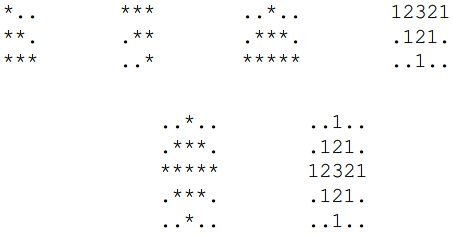
\includegraphics[width=90mm]{image/chapter_2/pyramid.jpg}
	\caption{কিছু পিরামিড $n = 3$ এর জন্য}
	\label{fig:pyramid}
\end{figure}

\section{সমীকরন}

\begin{align*}
& 1 + (1 + 2) + (1 + 2 + 3) + \ldots + (1 + 2 + \ldots + n) \\
&= \sum_{i = 1}^{n} {\sum_{j = 1}^{i} {j}} \\
&= \sum_{i = 1}^{n} { \frac{i^2 + i}{2} } \\
&= \frac{1}{2} \left( \sum_{i = 1}^{n} {i^2} + \sum_{i = 1}^{n} {i} \right) \\
&= \frac{1}{2} \left( \frac{n(n + 1)(2n + 1)}{6} + \frac{n^2 + n}{2} \right)
\end{align*}

বিগ-ও-নোটেশনের জন্য কাস্টম স্টাইলিং যেমন: আমরা লুপ ব্যবহার না করে শুধু কিছু যোগ আর গুণ করেই করে ফেলতে পারি, একে বলা হয় \BigO{1} অ্যালগরিদম।

তোমরা আশা করি ফিবোনাচি সংখ্যার(Fibonacci Number) কথা শুনেছ। যারা শুনো নাই তাদের জন্য বলি, $n$তম ফিবোনাচি সংখ্যাকে $F_n$ দিয়ে প্রকাশ করা হয়। এর মান:

\[
	F_n =
	\begin{cases}
		0  & n = 0 \\
		1 & n = 1 \\
		F_{n - 1} + F_{n - 2} & n \geq 2
	\end{cases}
\]

\section{কোটেশন}

{\fontfamily{uncl}\selectfont
\begin{quotation}
I learned a second lesson in the 60s, when I taught a course on programming to sophomores and discovered to my surprise that 10\% of my audience had the greatest difficulty in coping with the concept of recursive procedures. I was surprised because I knew that the concept of recursion was not difficult. Walking with my five-year old son through Eindhover, he suddenly said ``Dad, not every boat has a life-boat, has it?" ``How come?" I said. ``Well, the life-boat could have a smaller life-boat, but then that would be without one." It turned out.
\end{quotation}
}

\section{ম্যাট্রিক্স}

ম্যাট্রিক্স ব্যবহার করে আমরা লিখতে পারি:

\begin{align*}
\begin{bmatrix} F _2 \\ F_1 \end{bmatrix} &= \begin{bmatrix} 1 & 1 \\ 1 & 0 \end{bmatrix} \begin{bmatrix} F_1 \\ F_0 \end{bmatrix} \\
\begin{bmatrix} F _3 \\ F_2 \end{bmatrix} &= \begin{bmatrix} 1 & 1 \\ 1 & 0 \end{bmatrix} \begin{bmatrix} F_2 \\ F_1 \end{bmatrix} \\
&= \begin{bmatrix} 1 & 1 \\ 1 & 0 \end{bmatrix} \begin{bmatrix} 1 & 1 \\ 1 & 0 \end{bmatrix} \begin{bmatrix} F_1 \\ F_0 \end{bmatrix} \\
&= \begin{bmatrix} 1 & 1 \\ 1 & 0 \end{bmatrix}^2 \begin{bmatrix} F_1 \\ F_0 \end{bmatrix} \\
\end{align*}

একইভাবে,
\begin{align*}
\begin{bmatrix} F _4 \\ F_3 \end{bmatrix} = \begin{bmatrix} 1 & 1 \\ 1 & 0 \end{bmatrix}^3 \begin{bmatrix} F_1 \\ F_0 \end{bmatrix} \\
\end{align*}

সুতরাং আমরা লিখতে পারি,
\begin{align*}
\begin{bmatrix} F _n \\ F_{n-1} \end{bmatrix} = \begin{bmatrix} 1 & 1 \\ 1 & 0 \end{bmatrix}^{n-1} \begin{bmatrix} F_{1} \\ F_{0} \end{bmatrix} \\
\end{align*}


\section{একাধিক পৃষ্ঠায় বিস্তৃত টেবিল}


\begin{center}
\begin{longtable}{|c|c|c|}
\caption{গাউসের এলিমিনেশনের উদাহরণ\label{tab:gaussbig}} \\

\hline
\multicolumn{1}{|c|}{\textbf{Operation}} & \multicolumn{1}{c|}{\textbf{Equations}} & \multicolumn{1}{c|}{\textbf{Matrix}}\\
\hline 
\endfirsthead

\multicolumn{3}{c}
{{\bfseries \tablename\ \thetable{} -- পূর্বের পাতা থেকে}} \\
\hline \multicolumn{1}{|c|}{\textbf{Operation}} &
\multicolumn{1}{c|}{\textbf{Equations}} &
\multicolumn{1}{c|}{\textbf{Matrix}} \\ \hline 
\endhead

\multicolumn{3}{|r|}{{পরের পাতায় চলমান}} \\ \hline
\endfoot

\hline
\endlastfoot
শুরু & $\begin{array}{c} 2x -y +3z = 15 \\ 4x -2y +2z = 42 \\ x +y -z = 9 \end{array}$ & $\left[\begin{array}{ccc} 2 & -1 & 3 \\ 4 & -2 & 2 \\ 1 & 1 & -1 \end{array}\right] \left[ \begin{array}{c} x \\ y \\ z \end{array}\right] = \left[ \begin{array}{c} 15 \\ 42 \\ 9 \end{array}\right]$\\[20pt] 
\hline
$\frac{E_1}{2}$ & $\begin{array}{c} x -\frac{1}{2}y +\frac{3}{2}z = \frac{15}{2} \\ 4x -2y +2z = 42 \\ x +y -z = 9 \end{array}$ & $\left[\begin{array}{ccc} 1 & -\frac{1}{2} & \frac{3}{2} \\ 4 & -2 & 2 \\ 1 & 1 & -1 \end{array}\right] \left[ \begin{array}{c} x \\ y \\ z \end{array}\right] = \left[ \begin{array}{c} \frac{15}{2} \\ 42 \\ 9 \end{array}\right]$\\[20pt] 
\hline
$E_2 - 4E_1$ & $\begin{array}{c} x -\frac{1}{2}y +\frac{3}{2}z = \frac{15}{2} \\ -4z = 12 \\ x +y -z = 9 \end{array}$ & $\left[\begin{array}{ccc} 1 & -\frac{1}{2} & \frac{3}{2} \\ 0 & 0 & -4 \\ 1 & 1 & -1 \end{array}\right] \left[ \begin{array}{c} x \\ y \\ z \end{array}\right] = \left[ \begin{array}{c} \frac{15}{2} \\ 12 \\ 9 \end{array}\right]$\\[20pt] 
\hline
$E_3 - E_1$ & $\begin{array}{c} x -\frac{1}{2}y +\frac{3}{2}z = \frac{15}{2} \\ -4z = 12 \\ +\frac{3}{2}y -\frac{5}{2}z = \frac{3}{2} \end{array}$ & $\left[\begin{array}{ccc} 1 & -\frac{1}{2} & \frac{3}{2} \\ 0 & 0 & -4 \\ 0 & \frac{3}{2} & -\frac{5}{2} \end{array}\right] \left[ \begin{array}{c} x \\ y \\ z \end{array}\right] = \left[ \begin{array}{c} \frac{15}{2} \\ 12 \\ \frac{3}{2} \end{array}\right]$\\[20pt] 
\hline
$E_2 \leftrightarrow E_3$ & $\begin{array}{c} x -\frac{1}{2}y +\frac{3}{2}z = \frac{15}{2} \\ +\frac{3}{2}y -\frac{5}{2}z = \frac{3}{2} \\ -4z = 12  \end{array}$ & $\left[\begin{array}{ccc} 1 & -\frac{1}{2} & \frac{3}{2} \\ 0 & \frac{3}{2} & -\frac{5}{2} \\ 0 & 0 & -4 \end{array}\right] \left[ \begin{array}{c} x \\ y \\ z \end{array}\right] = \left[ \begin{array}{c} \frac{15}{2} \\ \frac{3}{2} \\ 12 \end{array}\right]$\\[20pt] 
\hline
$\frac{2E_2}{3}$ & $\begin{array}{c} x -\frac{1}{2}y +\frac{3}{2}z = \frac{15}{2} \\ y -\frac{5}{3}z = 1 \\ -4z = 12  \end{array}$ & $\left[\begin{array}{ccc} 1 & -\frac{1}{2} & \frac{3}{2} \\ 0 & 1 & -\frac{5}{3} \\ 0 & 0 & -4 \end{array}\right] \left[ \begin{array}{c} x \\ y \\ z \end{array}\right] = \left[ \begin{array}{c} \frac{15}{2} \\ 1 \\ 12 \end{array}\right]$\\[20pt] 
\hline
$E_1 + \frac{E_2}{2}$ & $\begin{array}{c} x +\frac{2}{3}z = 8 \\ y -\frac{5}{3}z = 1 \\ -4z = 12  \end{array}$ & $\left[\begin{array}{ccc} 1 & 0 & \frac{2}{3} \\ 0 & 1 & -\frac{5}{3} \\ 0 & 0 & -4 \end{array}\right] \left[ \begin{array}{c} x \\ y \\ z \end{array}\right] = \left[ \begin{array}{c} 8 \\ 1 \\ 12 \end{array}\right]$\\[20pt] 
\hline
$\frac{E_3}{-4}$ & $\begin{array}{c} x +\frac{2}{3}z = 8 \\ y -\frac{5}{3}z = 1 \\ z = -3  \end{array}$ & $\left[\begin{array}{ccc} 1 & 0 & \frac{2}{3} \\ 0 & 1 & -\frac{5}{3} \\ 0 & 0 & 1 \end{array}\right] \left[ \begin{array}{c} x \\ y \\ z \end{array}\right] = \left[ \begin{array}{c} 8 \\ 1 \\ -3 \end{array}\right]$\\[20pt] 
\hline
$E_1 - \frac{2E_3}{3}$ & $\begin{array}{c} x = 10 \\ y -\frac{5}{3}z = 1 \\ z = -3  \end{array}$ & $\left[\begin{array}{ccc} 1 & 0 & 0 \\ 0 & 1 & -\frac{5}{3} \\ 0 & 0 & 1 \end{array}\right] \left[ \begin{array}{c} x \\ y \\ z \end{array}\right] = \left[ \begin{array}{c} 10 \\ 1 \\ -3 \end{array}\right]$\\[20pt] 
\hline
$E_2 + \frac{5E_3}{3}$ & $\begin{array}{c} x = 10 \\ y = -4 \\ z = -3  \end{array}$ & $\left[\begin{array}{ccc} 1 & 0 & 0 \\ 0 & 1 & 0 \\ 0 & 0 & 1 \end{array}\right] \left[ \begin{array}{c} x \\ y \\ z \end{array}\right] = \left[ \begin{array}{c} 10 \\ -4 \\ -3 \end{array}\right]$\\[20pt]
\end{longtable}
\end{center}


\section{সিমুলেশন}

সাধারণত আমরা বাস্তবে এভাবে সর্টিং করে থাকি। মনে কর আমাদের কাছে $60$ জনের খাতা আছে। আমরা একটি করে খাতা নেই, আর ক্রমানুসারে সাজানো বা সর্টেড খাতাগুলোর মধ্যে এই খাতাকে সঠিক জায়গায় রাখি। আবার নতুন খাতা নিব আর ক্রমানুসারে সাজানো খাতাগুলোর মধ্যে এই নতুন খাতাকে ঠিক জায়গায় রাখব। এভাবে সবগুলো খাতাকে রাখা শেষ হলেই আমাদের সর্টিংও শেষ হয়ে যাবে। এখন যদি ইমপ্লিমেন্টেশনের কথা চিন্তা কর তাহলে মনে হবে এভাবে একটি একটি করে খাতা ঢুকানো মনে হয় কঠিন কাজ। কিন্তু ওত কঠিন না। মনে কর তোমার $1 \ldots i-1$ খাতাগুলো সাজানো আছে, তুমি $i$ তম খাতা ঢুকাবে, তুমি প্রথমে দেখ $i-1$ এর খাতাটি কি তোমার থেকে ছোট? তাহলে যেখানে আছে সেখানেই তোমার খাতার অবস্থান আর যদি না হয় তাহলে $i-1$ এ থাকা খাতাকে $i$ এ আনো আর এবার $i-2$ এর সঙ্গে মিলিয়ে দেখো। এভাবে একে একে তুলনা করতে থাক। একটি উদাহরণ টেবিল \ref{tab:insertion} এ দেওয়া হলো।

এর কোডটিও কিন্তু বেশ ছোট। কিন্তু কোড করতে সোজা হলেও এই অ্যালগরিদমের টাইম কমপ্লেক্সিটি \BigO{n^2}. আমরা পরে দেখব এর থেকেও অনেক দ্রুত সর্টিং করা সম্ভব।

অর্থহীন লেখা যার মাঝে আছে অনেক কিছু। হ্যাঁ, এই লেখার মাঝেই আছে অনেক কিছু। যদি তুমি মনে করো, এটা তোমার কাজে লাগবে, তাহলে তা লাগবে কাজে। নিজের ভাষায় লেখা দেখতে অভ্যস্ত হও। মনে রাখবে লেখা অর্থহীন হয়, যখন তুমি তাকে অর্থহীন মনে করো; আর লেখা অর্থবোধকতা তৈরি করে, যখন তুমি তাতে অর্থ ঢালো। যেকোনো লেখাই তোমার কাছে অর্থবোধকতা তৈরি করতে পারে, যদি তুমি সেখানে অর্থদ্যোতনা দেখতে পাও। ...ছিদ্রান্বেষণ? না, তা হবে কেন?

যে কথাকে কাজে লাগাতে চাও, তাকে কাজে লাগানোর কথা চিন্তা করার আগে ভাবো, তুমি কি সেই কথার জাদুতে আচ্ছন্ন হয়ে গেছ কিনা। তুমি যদি নিশ্চিত হও যে, তুমি কোনো মোহাচ্ছাদিত আবহে আবিষ্ট হয়ে অন্যের শেখানো বুলি আত্মস্থ করছো না, তাহলে তুমি নির্ভয়ে, নিশ্চিন্তে অগ্রসর হও। তুমি সেই কথাকে জানো, বুঝো, আত্মস্থ করো; মনে রাখবে, যা অনুসরণ করতে চলেছো, তা আগে অনুধাবন করা জরুরি; এখানে কিংকর্তব্যবিমূঢ় হবার কোনো সুযোগ নেই।


\begin{table}[!hbt]
	\caption{ইনসার্শন সর্টের সিমুলেশন \label{tab:insertion}}
	\renewcommand{\arraystretch}{2}
	\begin{center}
	\begin{tabular}{|c|}
		\hline
		{\large \textcircled{\small 5}}, 8, 6, 1, 7, 9 \\\hline 
		\boxed{5}, {\large \textcircled{\small 8}}, 6, 1, 7, 9 \\\hline
		\boxed{5}, \boxed{8}, {\large \textcircled{\small 6}}, 1, 7, 9 \\\hline
		\boxed{5}, {\large \textcircled{\small 6}}, \boxed{8}, 1, 7, 9 \\\hline
		\boxed{5}, \boxed{6}, \boxed{8},  {\large \textcircled{\small 1}}, 7, 9 \\\hline
		\boxed{5}, \boxed{6}, {\large \textcircled{\small 1}}, \boxed{8}, 7, 9 \\\hline
		\boxed{5}, {\large \textcircled{\small 1}}, \boxed{6}, \boxed{8}, 7, 9 \\\hline
		 {\large \textcircled{\small 1}}, \boxed{5}, \boxed{6}, \boxed{8}, 7, 9 \\\hline
		\boxed{1}, \boxed{5}, \boxed{6}, \boxed{8}, {\large \textcircled{\small 7}}, 9 \\\hline
		\boxed{1}, \boxed{5}, \boxed{6}, {\large \textcircled{\small 7}}, \boxed{8}, 9 \\\hline
		\boxed{1}, \boxed{5}, \boxed{6}, \boxed{7}, \boxed{8},  {\large \textcircled{\small 9}} \\\hline
		\boxed{1}, \boxed{5}, \boxed{6}, \boxed{7}, \boxed{8}, \boxed{9} \\\hline
	\end{tabular}
	\end{center}
\end{table}



\section{ইপিএস (eps) ছবি}

বাইনারি সার্চ ব্যবহার করে কিছু অদ্ভুত সমস্যাও সমাধান করা যায়। অদ্ভুত বললাম এই কারণে যে, প্রবলেম দেখে হয়তো কখনই মনে হবে না যে এখানে বাইনারি সার্চ ব্যবহার করা যায়, কিন্তু যায়! যেমন ~\ref{fig:ladder} নং চিত্রে একটি $w$ প্রস্থের রাস্তার দুদিকে দুটি দালান আছে। এখন রাস্তার এক মাথায় একটি মই রেখে অপর মাথা রাস্তার অন্য পারের দালানের মাথায় রাখা হলো, একইভাবে রাস্তার অন্য পাশ থেকেও আরেকটি মই রাখা হলো। মই দুটির দৈর্ঘ্য $a$ ও $b$. মই দুটি রাস্তা থেকে $c$ উচ্চতায় ছেদ করে। $a, b$ এবং $c$ এর মান দেওয়া আছে, $w = ?$.

\begin{figure}[ht!]
	\centering
	
\includegraphics[width=40mm]{image/chapter_2/ladder.eps}
	\caption{w = ?}
	\label{fig:ladder}
\end{figure}

\section{কাস্টম ছবি}

মনে করি আমাদের দাবা বোর্ডের সারিগুলো উপর থেকে নিচে $1$ হতে $8$ পর্যন্ত নম্বর করা এবং কলামগুলো বাম থেকে ডান দিকে $1$ হতে $8$ পর্যন্ত নম্বর করা (চিত্র ~\ref{fig:chess})। এখন একটু খেয়াল করলে দেখবে যেসব কর্ণ উপরের বাম দিক থেকে নিচের ডান দিকে যায় সেসব কর্ণে থাকা ঘরগুলোর সারি ও কলামের বিয়োগফল একই হয় এবং যেসব কর্ণ উপরের ডান দিক থেকে নিচের বাম দিকে যায় তাতে থাকা ঘরগুলোর সারি ও কলামের যোগফল একই হয়। 

		\begin{figure}[ht!]
			\centering
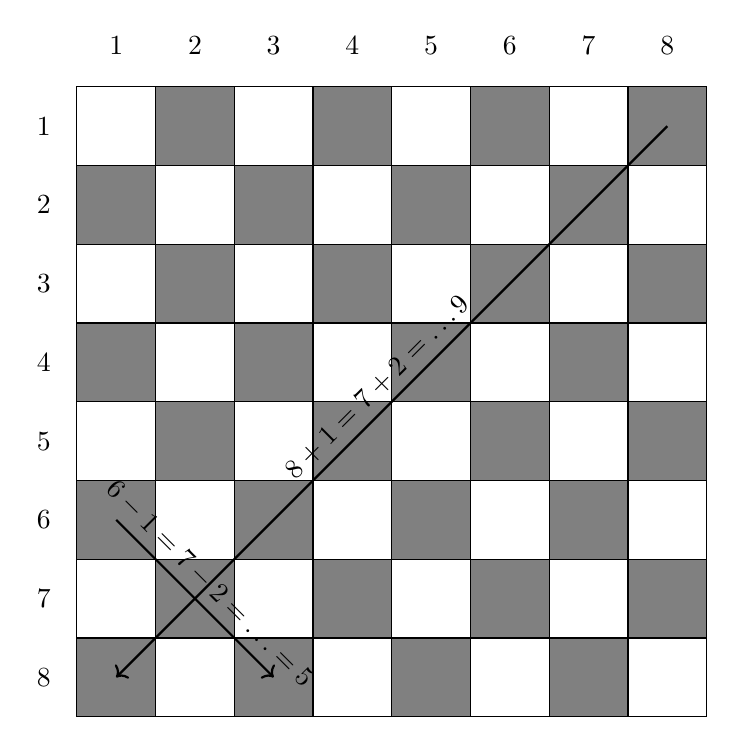
\begin{tikzpicture}
    \pgfmathsetmacro{\boardsize}{8}

    \def\letters{{"","8","7","6","5","4","3","2","1","i","j","k","l","m","n","o","p","q","r","s","t","u","v","w","x","y","z"}}

    \foreach \i in {1,...,\boardsize}{
        \foreach \j in {1,...,\boardsize}{
            \pgfmathsetmacro{\weight}{(1 + (-1)^(\i+\j))*50};
            \node[draw=black,rectangle,fill=gray!\weight,minimum size=1cm] (node\i-\j) at (\i,\j) {};
        }
    }
    \foreach \j in {1,...,\boardsize}{
        \node[left=2mm of node1-\j] {\pgfmathparse{\letters[\j]}\pgfmathresult};
    }

    \foreach \i in {1,...,\boardsize}{
        \node[above=4mm of node\i-\boardsize,anchor=base] {\i};
    }
    
    \draw[thick,->] (8, 8) -- (1, 1) node [midway, above, sloped] {$8 + 1 = 7 + 2 = \ldots 9$};
    \draw[thick,->] (1, 3) -- (3, 1) node [midway, above, sloped] {$6 - 1 = 7 - 2 = \ldots = 5$};
 
\end{tikzpicture}
			\caption{দাবা বোর্ড}
			\label{fig:chess}
		\end{figure}
		
অর্থহীন লেখা যার মাঝে আছে অনেক কিছু। হ্যাঁ, এই লেখার মাঝেই আছে অনেক কিছু। যদি তুমি মনে করো, এটা তোমার কাজে লাগবে, তাহলে তা লাগবে কাজে। নিজের ভাষায় লেখা দেখতে অভ্যস্ত হও। মনে রাখবে লেখা অর্থহীন হয়, যখন তুমি তাকে অর্থহীন মনে করো; আর লেখা অর্থবোধকতা তৈরি করে, যখন তুমি তাতে অর্থ ঢালো। যেকোনো লেখাই তোমার কাছে অর্থবোধকতা তৈরি করতে পারে, যদি তুমি সেখানে অর্থদ্যোতনা দেখতে পাও। ...ছিদ্রান্বেষণ? না, তা হবে কেন?

যে কথাকে কাজে লাগাতে চাও, তাকে কাজে লাগানোর কথা চিন্তা করার আগে ভাবো, তুমি কি সেই কথার জাদুতে আচ্ছন্ন হয়ে গেছ কিনা। তুমি যদি নিশ্চিত হও যে, তুমি কোনো মোহাচ্ছাদিত আবহে আবিষ্ট হয়ে অন্যের শেখানো বুলি আত্মস্থ করছো না, তাহলে তুমি নির্ভয়ে, নিশ্চিন্তে অগ্রসর হও। তুমি সেই কথাকে জানো, বুঝো, আত্মস্থ করো; মনে রাখবে, যা অনুসরণ করতে চলেছো, তা আগে অনুধাবন করা জরুরি; এখানে কিংকর্তব্যবিমূঢ় হবার কোনো সুযোগ নেই।


\section{গ্রাফ}
অ্যালগরিদম হচ্ছে একটি সমস্যা সমাধানের পথ আর ডেটা স্ট্রাকচার (Data Structure) হচ্ছে ডেটাকে সাজিয়ে রাখার জিনিস। অনেক সময় কোনো একটি অ্যালগরিদমের এফিসিয়েন্সি (efficiency) ডেটা স্ট্রাকচারের উপর নির্ভর করে। খুব সহজ একটি উদাহরণ দেয়া যাক। মনে কর তোমাকে একে একে একটি করে সংখ্যা দেওয়া হবে $1$ থেকে $n$ এর মধ্যে, তোমাকে বলতে হবে এই সংখ্যাটা এর আগে এসেছিল কিনা। তুমি কীভাবে করবে? একটি উপায় হলো সংখ্যার একটি অ্য়ারে রাখা। যখন কোনো সংখ্যা আসবে তখন ওই অ্যারেতে খুঁজে দেখ এর আগে ওই সংখ্যা এসেছিল কিনা যদি না থাকে তাহলে এই অ্যারের শেষে এই সংখ্যাটা রাখ। আরেকটি উপায় হলো এমন একটি অ্যারে রাখ যেখানে তোমার লেখা থাকবে যে কোনো একটি সংখ্যা এর আগে এসেছিল কিনা। খেয়াল কর এখানে তুমি সংখ্যাগুলো রাখবে না শুধু কোনো একটি সংখ্যা এসেছিল কিনা তা রাখবে।

\newsavebox{\tempbox}

\begin{figure}
% store the bigger of the two pictures in a vbox
\sbox{\tempbox}{%
    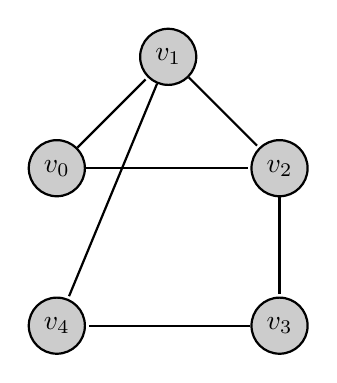
\begin{tikzpicture}[-,>=stealth',shorten >=1pt,auto,node distance=2cm,
      thick,main node/.style={circle,fill=black!20,draw}]

      \node[main node] (1) {$v_1$};
      \node[main node] (2) [below left of=1] {$v_0$};
      \node[main node] (3) [below right of=1] {$v_2$};
      \node[main node] (4) [below of=3] {$v_3$};
      \node[main node] (5) [below of=2] {$v_4$};

      \path[every node/.style={font=\sffamily\small}]
        (2) edge node [left] {} (1)
        (2) edge node [left] {} (3)
        (1) edge node [left] {} (5)
        (1) edge node [left] {} (3)
        (3) edge node [left] {} (4)
        (4) edge node [left] {} (5)
        ;
    \end{tikzpicture}
}
\begin{subfigure}{.5\textwidth}
    \centering
    \usebox{\tempbox}
\caption{গ্রাফ (Graph)}
\end{subfigure}%
\begin{subfigure}{.5\textwidth}
    \centering
    \vbox to\ht\tempbox{
        \vfill
    \begin{math}
    \left(
    \begin{array}{ccccc}
    0 & 1 & 1 & 0 & 0 \\
    1 & 0 & 1 & 0 & 1 \\
    1 & 1 & 0 & 1 & 0 \\
    0 & 0 & 1 & 0 & 1 \\
    0 & 1 & 0 & 1 & 0
    \end{array}
    \right)
    \end{math}
    \vfill
    }
    \caption{অ্যাডজাসেন্সি ম্যাট্রিক্স (Adjacency Matrix)}
\end{subfigure}%
\caption{একটি গ্রাফের অ্যাডজাসেন্সি ম্যাট্রিক্সের উপস্থাপন}
			\label{fig:adjmat}
\end{figure}

\section{রঙ্গীন ছবি}

এটিও বেশ সহজ অ্যালগরিদম। কোনো কারণে যখনই MST আমাকে কোড করতে হয় আমি ক্রুসকাল এর অ্যালগরিদম (Kruskal's algorithm) ই করে থাকি। হয়তো আমার কাছে এটি সহজ লাগে সেজন্য! এই অ্যালগরিদম বোঝানো খুবই সহজ, কোড করাও অনেক সহজ কিন্তু যেভাবে কোড করতে হবে সেটি বোঝানো একটু কষ্টকর। এই অ্যালগরিদমে তুমি যা করবে তাহলো সবচেয়ে কম ওজনের বাহু নিবে, দেখবে এর দুই মাথার ভার্টেক্স দুটি ইতোমধ্যেই একই ট্রি বা component এ আছে কিনা, থাকলে এই বাহু নিবে না। না থাকলে নিবে। এভাবে মূল্যের ঊর্ধ্বক্রমে সব বাহুর ইউনিয়ন (union) নিয়ে এই কাজ করতে হবে। শেষ! এখন প্রশ্ন হচ্ছে কীভাবে বুঝবে যে দুটি ভার্টেক্স একই ট্রি তে আছে কিনা! উত্তর: ডিসজয়েন্ট সেট (Disjoint Set) . প্রথমে সব ভার্টেক্সকে আলাদা আলাদা সেট আকারে কল্পনা কর। আমরা যখনই একটি বাহু নিচ্ছি তখন দুটি সেটকে জোড়া লাগানোর চেষ্টা করছি এবং সেজন্য যাচাই করছি যে, এই দুটি ভার্টেক্স একই সেটে আছে কিনা! 

\begin{figure}[ht!]
\centering
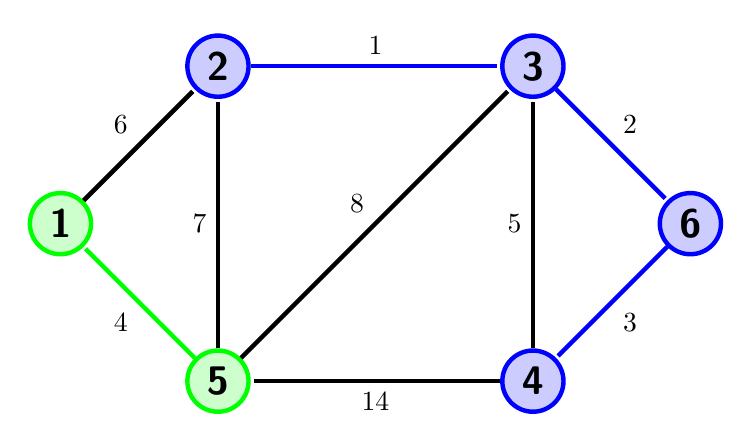
\begin{tikzpicture}[shorten >=1pt, auto, node distance=3cm, ultra thick,
    node_style/.style={circle,draw=green,fill=green!20!,font=\sffamily\Large\bfseries},
    selected_node_style/.style={circle,draw=blue,fill=blue!20!,font=\sffamily\Large\bfseries},
    edge_style/.style={draw=black, ultra thick},
    selected_edge_style/.style={draw=blue, ultra thick},
    selected_edge_style2/.style={draw=green, ultra thick}]

    \node[node_style] (v1) at (-4,0) {1};
    \node[selected_node_style] (v2) at (-2,2) {2};
    \node[selected_node_style] (v3) at (2,2) {3};
    \node[selected_node_style] (v4) at (2,-2) {4};
    \node[node_style] (v5) at (-2,-2) {5};
    \node[selected_node_style] (v6) at (4,0) {6};

    \draw[selected_edge_style]  (v2) edge node{1} (v3);
    \draw[selected_edge_style]  (v3) edge node{2} (v6);
    \draw[selected_edge_style]  (v6) edge node{3} (v4);
    \draw[edge_style]  (v4) edge node{14} (v5);
    \draw[selected_edge_style2]  (v5) edge node{4} (v1);
    \draw[edge_style]  (v1) edge node{6} (v2);
    \draw[edge_style]  (v5) edge node{7} (v2);
    \draw[edge_style]  (v5) edge node{8} (v3);
    \draw[edge_style]  (v4) edge node{5} (v3);
\end{tikzpicture}
\caption{ক্রুসকাল এর অ্যালগরিদম (Kruskal's algorithm)}
\label{fig:kruskal}
\end{figure}

একটি উদাহরণ দেখা যাক। চিত্র ~\ref{fig:kruskal} এ আমরা প্রথমে $2-3$ কে জোড়া দিয়েছি। এরপর $3-6$, $6-4$, $1-5$. ওজনের ঊর্ধ্বক্রমে আসলে আমাদের পরের বাহু হবে $3-4$ কিন্তু এই দুটি নোড একই ট্রি তে আছে সুতরাং আমরা আর এই বাহু জোড়া লাগাব না। এর পরের বাহু হলো $1-2$ এবং এটি দুটি আলাদা ট্রি কে জোড়া লাগায় সুতরাং আমরা এই বাহু নিব এবং ট্রি দুটিকে জোড়া লাগাব। অর্থাৎ যদি ডিসজয়েন্ট সেট ইউনিয়নের ভাষায় বলতে হয়, তাহলে প্রথমে আমরা বাহুগুলোকে মূল্য অনুযায়ী ছোট হতে বড় আকারে সাজাবো। এরপর তাদের একে একে নিবো আর দেখবো এই বাহুর দুই মাথা একই সেটে আছে কি না। থাকলে এই বাহু নিবো না। আর না থাকলে সেই বাহু নেবো আর তাদের দুই মাথার সেটগুলো ইউনিয়ন করে দেব।

এখন প্রশ্ন হলো এই অ্যালগরিদমের টাইম কমপ্লেক্সিটি কত? সহজ, বাহুগুলোকে ওজন অনুযায়ী সর্ট করতে \BigO{m\log{m}} এবং প্রতি বাহুর জন্য আমরা ফাইন্ড (find) করছি বা দুটি সেটকে ইউনিয়ন করছি যাদের কমপ্লেক্সিটি আমরা \BigO{1} ধরে নিতে পারি। সুতরাং \BigO{m\log{m} + m} = \BigO{m\log{m}}.



\begin{figure}[ht!]
\centering
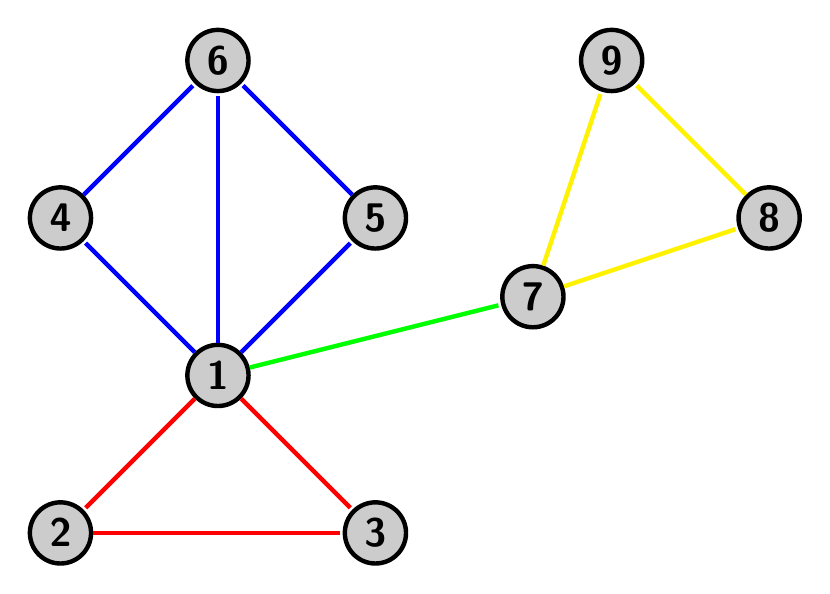
\begin{tikzpicture}[shorten >=1pt, auto, node distance=3cm, ultra thick,
    node_style/.style={circle,draw=black,fill=black!20!,font=\sffamily\Large\bfseries},
    edge_style1/.style={draw=red, ultra thick},
    edge_style2/.style={draw=blue, ultra thick},
    edge_style3/.style={draw=green, ultra thick},
    edge_style4/.style={draw=yellow, ultra thick}]

	\node[node_style] (v1) at (0, 0) {1};
	\node[node_style] (v2) at (-2, -2) {2};
	\node[node_style] (v3) at (2, -2) {3};
	\node[node_style] (v4) at (-2, 2) {4};
	\node[node_style] (v5) at (2, 2) {5};
	\node[node_style] (v6) at (0, 4) {6};
	\node[node_style] (v7) at (4, 1) {7};
	\node[node_style] (v8) at (7, 2) {8};
	\node[node_style] (v9) at (5, 4) {9};

	\draw[edge_style1] (v1) edge node{} (v2);
	\draw[edge_style1] (v1) edge node{} (v3);
	\draw[edge_style1] (v2) edge node{} (v3);
	
	\draw[edge_style2] (v1) edge node{} (v4);
	\draw[edge_style2] (v1) edge node{} (v5);
	\draw[edge_style2] (v1) edge node{} (v6);
	\draw[edge_style2] (v4) edge node{} (v6);
	\draw[edge_style2] (v5) edge node{} (v6);

	\draw[edge_style3] (v1) edge node{} (v7);
	
	\draw[edge_style4] (v7) edge node{} (v8);
	\draw[edge_style4] (v7) edge node{} (v9);
	\draw[edge_style4] (v8) edge node{} (v9);
\end{tikzpicture}
\caption{বাইকানেক্টেড অ্যালগরিদম (Biconnected algorithm)}
\label{fig:bcc}
\end{figure}

তোমরা চিত্র ~\ref{fig:bcc} এ যদি বলতে প্রতিটি বাহু আলাদা আলাদা কম্পোনেন্ট, হ্যাঁ কথা ঠিক কিন্তু এই যে বললাম প্রতিটি কম্পোনেন্টকে আমরা বড় করার চেষ্টা করি, সে জন্য আমাদের BCC হবে চিত্রের মতো।



%\clearpage \addcontentsline{toc}{chapter}{Index} \printindex

\end{document}

